% The hardest textbook exercises on the topics of Listas 1-7: list + solutions.
% Plan (references, weights, readings): pratica-hardest.md. Statements are NOT reproduced (CLAUDE.md).
% Romer solutions: hardest-parts/*.tex, each checked by hardest-parts/*-check.py.
% Compile: pdflatex (2x); check: pdffonts (all Type 1).
\documentclass[11pt,a4paper]{article}
% Shared preamble of the answer key to the hardest textbook exercises (hardest-solutions.tex).
% Fragments in hardest-parts/*.tex use only the macros below. Statements are NOT reproduced
% (CLAUDE.md): each solution cites the exercise by number and page.
\usepackage[utf8]{inputenc}
\usepackage[T1]{fontenc}
\usepackage{lmodern}   % Type 1 vector fonts (replaces PK bitmaps)
\usepackage{cmap}      % ToUnicode CMap -> copyable text and accents
\usepackage[english]{babel}
\usepackage{amsmath,amssymb,amsfonts}
\usepackage[a4paper,margin=2.2cm]{geometry}
\usepackage{enumitem}
\usepackage{fancyhdr}
\usepackage{xcolor}
\usepackage{microtype}
\usepackage{booktabs}
\usepackage{longtable}
\usepackage{tikz}
\usepackage[hidelinks]{hyperref}

\pagestyle{fancy}\fancyhf{}
\lhead{\footnotesize Macroeconomics I --- MPE Insper}
\rhead{\footnotesize Hardest textbook exercises --- solutions}
\cfoot{\footnotesize\thepage}
\renewcommand{\headrulewidth}{0.3pt}
\setlength{\headheight}{14pt}
\setlist{topsep=2pt,itemsep=2pt}

% \problema{Romer 1.12}{Embodied technological progress}{p.~47--48}{Romer \S1.3, \S1.5}
\newcommand{\problema}[4]{\bigskip\noindent
  {\large\bfseries\color{blue!55!black}#1 --- #2}\par\nopagebreak
  \noindent{\footnotesize\color{black!60}Statement in the book, #3. Background: #4.}\par
  \noindent\rule{\linewidth}{0.3pt}\par\nopagebreak\smallskip
  \addcontentsline{toc}{subsection}{#1 --- #2}}
\newcommand{\parte}[1]{\par\medskip\noindent\textbf{(#1)}\ }
\newcommand{\passo}[2]{\par\smallskip\noindent\textbf{Step --- #1.}~#2}
\newcommand{\intuicao}[1]{\par\smallskip\noindent\textit{Economic intuition.}~#1}
\newcommand{\armadilha}[1]{\par\smallskip\noindent\textit{Where this goes wrong.}~#1}
\newcommand{\refbib}[1]{\par\smallskip\noindent{\footnotesize\color{black!60}\textbf{Ref:} #1}}
\newcommand{\checado}[1]{\par\smallskip\noindent{\footnotesize\color{black!60}\textbf{Checked:} #1}}


\begin{document}
\begin{center}
  {\Large\bfseries Macroeconomics I --- MPE Insper}\\[2pt]
  {\large The hardest textbook exercises on Listas 1--7: list and solutions}
\end{center}

\noindent\textbf{How to use this.} Thirty exercises from Kurlat (2020) and Romer (2012), the hardest
the two books offer on the course's topics. Statements are not reproduced: open the book at the
page given and attempt the exercise fully before reading the solution. Kurlat's exercises are solved
step by step, with verification code, in the existing \texttt{Resolucao/kurlat\_solutions\_*.pdf}
(the page column below is the PDF page). Romer's problems are solved in Part~II of this document;
every number and key derivation there is re-checked by the scripts in \texttt{Listas/hardest-parts/}.
Weights, readings and the study roadmap are in \texttt{Listas/pratica-hardest.md}.

\section*{Part I --- The list}
\addcontentsline{toc}{section}{Part I --- The list}

{\small
\begin{longtable}{@{}rllllll@{}}
\toprule
\# & Book & No. & Page & Topic & Level & Solution \\
\midrule
\endhead
1 & Kurlat & 2.7 & 42 & Welfare: risk aversion & Advanced & \texttt{ch1-4}, p.~29 \\
2 & Kurlat & 2.8 & 42 & Welfare: inequality & Advanced & \texttt{ch1-4}, p.~30 \\
3 & Kurlat & 2.9 & 43 & Welfare: cross-country & Advanced & \texttt{ch1-4}, p.~20 \\
4 & Kurlat & 2.10 & 43 & Welfare: difference principle & Advanced & \texttt{ch1-4}, p.~32 \\
5 & Kurlat & 4.4 & 73 & AK model & Advanced & \texttt{ch1-4}, p.~50 \\
6 & Kurlat & 4.5 & 73 & Malthusian model & Advanced & \texttt{ch1-4}, p.~53 \\
7 & Kurlat & 5.2 & 94 & Speed of convergence & Advanced & \texttt{ch05}, p.~7 \\
8 & Kurlat & 5.7 & 96 & Accounts, returns, growth accounting & Advanced & \texttt{ch05}, p.~13 \\
9 & Kurlat & 5.8 & 97 & Golden Rule from national accounts & Advanced & \texttt{ch05}, p.~16 \\
10 & Kurlat & 6.9 & 125 & Marginal propensity to consume & Advanced & \texttt{ch06}, p.~8 \\
11 & Kurlat & 7.5 & 148 & Prescott's calculation & Advanced & \texttt{ch07}, p.~14 \\
12 & Kurlat & 9.12 & 185 & Optimal vs fixed saving & Advanced & \texttt{ch09}, p.~30 \\
13 & Kurlat & 9.13 & 186 & First Welfare Theorem failure & Advanced & \texttt{ch09}, p.~16 \\
14 & Kurlat & 10.5 & 203 & Baumol--Tobin & Advanced & \texttt{ch10-11}, p.~8 \\
15 & Kurlat & 11.6 & 219 & Seignorage, Laffer curve & Advanced & \texttt{ch10-11}, p.~17 \\
16 & Kurlat & 11.7 & 221 & Bank seignorage & Advanced & \texttt{ch10-11}, p.~23 \\
17 & Romer & 1.12 & 47--48 & Embodied technical progress & Graduate & Part II \\
18 & Romer & 1.15 & 48 & Resources and land & Graduate & Part II \\
19 & Romer & 4.8 & 186 & Education sector & Graduate & Part II \\
20 & Romer & 8.1 & 398 & Life-cycle saving & Graduate & Part II \\
21 & Romer & 8.13 & 402--403 & Habit formation & Graduate & Part II \\
22 & Romer & 8.15 & 403--404 & Time inconsistency & Graduate & Part II \\
23 & Romer & 10.16 & 512 & Search efficiency & Graduate & Part II \\
24 & Romer & 2.9 & 95 & Closed-form Ramsey & Graduate & Part II \\
25 & Romer & 2.12 & 96 & Temporary capital taxes & Graduate & Part II \\
26 & Romer & 11.1 & 576 & Forward-looking Cagan & Graduate & Part II \\
27 & Romer & 11.22 & 583 & Adaptive-expectations Cagan & Graduate & Part II \\
28 & Romer & 6.16 & 311 & Flexible vs rigid prices & Graduate & Part II \\
29 & Romer & 6.10 & 308--309 & Menu costs, multiple equilibria & Graduate & Part II \\
30 & Romer & 6.7 & 308 & Liquidity trap & Graduate & Part II \\
\bottomrule
\end{longtable}}

\noindent{\footnotesize Book pages are printed pages: Kurlat (2020), \emph{A Course in Modern Macroeconomics};
Romer (2012), \emph{Advanced Macroeconomics}, 4th ed. Solution pages for Kurlat refer to the PDF pages of
\texttt{Resolucao/kurlat\_solutions\_<chapter>.pdf}.\par}

\tableofcontents

\section*{Part II --- Solutions to the Romer problems}
\addcontentsline{toc}{section}{Part II --- Solutions to the Romer problems}

% Romer (2012), Problem 1.12 --- solution fragment, \input by ../hardest-solutions.tex.
% Statement not reproduced (project rule). Every result is re-derived by check-1-12-1-15.py.
\problema{Romer 1.12}{Embodied technological progress}{pp.~47--48}{Romer \S1.3, \S1.5}
\noindent\textbf{Notation and assumptions.} $g_X\equiv\dot X/X$ for any variable $X$. Labor grows at
rate $n$ and $A$ at rate $\mu>0$; $0<\alpha<1$, $0<s<1$ and $n+\delta>0$. Throughout,
$\phi\equiv\alpha/(1-\alpha)$, so that $\alpha=\phi(1-\alpha)$ and $1+\phi=1/(1-\alpha)$.

\parte{a}
\passo{Capital-augmenting progress is labor-augmenting in disguise}{Because $\alpha=\phi(1-\alpha)$,
$A^{\alpha}=(A^{\phi})^{1-\alpha}$, and the production function can be rewritten as
\[ Y=A^{\alpha}K^{\alpha}L^{1-\alpha}=K^{\alpha}(A^{\phi}L)^{1-\alpha}
\quad\Longrightarrow\quad
y\equiv\frac{Y}{A^{\phi}L}=\Big(\frac{K}{A^{\phi}L}\Big)^{\alpha}=k^{\alpha},
\qquad k\equiv\frac{K}{A^{\phi}L}. \]}
\passo{Law of motion of $k$}{Log-differentiating the definition of $k$ gives $g_k=g_K-\phi\mu-n$.
Dividing $\dot K=sY-\delta K$ by $K$ gives $g_K=s\,Y/K-\delta$, and $Y/K=y/k=k^{\alpha-1}$. Hence
\[ \frac{\dot k}{k}=s\,k^{\alpha-1}-m_a,\qquad m_a\equiv n+\delta+\phi\mu>0,
\qquad\text{that is,}\qquad \dot k=s\,k^{\alpha}-m_a\,k. \]}
\passo{Global convergence}{The growth rate of $k$, $\Gamma_a(k)\equiv s\,k^{\alpha-1}-m_a$, satisfies
\[ \Gamma_a'(k)=-(1-\alpha)s\,k^{\alpha-2}<0,\qquad \lim_{k\downarrow0}\Gamma_a(k)=+\infty,\qquad
\lim_{k\to\infty}\Gamma_a(k)=-m_a<0. \]
So it has a unique zero, $k^*=(s/m_a)^{1/(1-\alpha)}$, with $\dot k>0$ for $k<k^*$ and $\dot k<0$ for $k>k^*$. From any $k(0)>0$, $k$ moves monotonically
toward $k^*$ and cannot cross it (it is a rest point), so $k(t)\to k^*$.}
\passo{Balanced growth}{At $k=k^*$, $y=y^*=(k^*)^{\alpha}$ is constant, so $K=k^*A^{\phi}L$ and
$Y=y^*A^{\phi}L$ both grow at the growth rate of $A^{\phi}L$:
\[ g_K^{\mathrm{bgp}}=g_Y^{\mathrm{bgp}}=n+\phi\mu=n+\frac{\alpha\mu}{1-\alpha},\qquad
g_{Y/L}^{\mathrm{bgp}}=g_{K/L}^{\mathrm{bgp}}=\frac{\alpha\mu}{1-\alpha}. \]}
\intuicao{With Cobb--Douglas technology it does not matter which factor $A$ multiplies: $A^{\alpha}$
on capital is $(A^{\phi})^{1-\alpha}$ on labor, so capital-augmenting progress at rate $\mu$ is
labor-augmenting progress at rate $\phi\mu$, and the Solow result (output per worker grows at the
rate of labor-augmenting progress) delivers $\alpha\mu/(1-\alpha)$. That is why the problem imposes
Cobb--Douglas: otherwise capital-augmenting progress is incompatible with balanced growth (Uzawa's
theorem).}

\parte{b}
\passo{Change of variable}{Let $\tilde J\equiv J/A$. Then $Y=J^{\alpha}L^{1-\alpha}=(A\tilde J)^{\alpha}
L^{1-\alpha}$, the technology of (a) with $\tilde J$ in place of $K$. As in (a),
$Y=\tilde J^{\alpha}(A^{\phi}L)^{1-\alpha}$, so $y\equiv Y/(A^{\phi}L)=j^{\alpha}$ with
$j\equiv\tilde J/(A^{\phi}L)$.}
\passo{Accumulation of $\tilde J$: obsolescence}{Using $\dot J=sAY-\delta J$ and $J=A\tilde J$,
\[ g_{\tilde J}=g_J-\mu=\frac{sAY}{J}-\delta-\mu=\frac{sY}{\tilde J}-(\delta+\mu)
\quad\Longrightarrow\quad \dot{\tilde J}=sY-(\delta+\mu)\tilde J. \]
This is the capital accumulation equation of (a) with depreciation rate $\delta+\mu$. Integrating,
\[ \tilde J(t)=e^{-(\delta+\mu)t}\,\tilde J(0)+\int_0^t e^{-(\delta+\mu)(t-v)}\,sY(v)\,dv: \]
one unit of output invested at $v$ still supplies $e^{-\delta(t-v)}A(v)$ units of $J$ at $t$, as
many as $e^{-(\delta+\mu)(t-v)}$ units of output invested at $t$ would. So $\tilde J$ measures the
stock in current-vintage machines, and it loses value through decay ($\delta$) and obsolescence
($\mu$).}
\passo{Law of motion of $j$}{Log-differentiating, $g_j=g_{\tilde J}-\phi\mu-n$. With
$Y/\tilde J=y/j=j^{\alpha-1}$ and $\mu+\phi\mu=\mu/(1-\alpha)$,
\[ \dot j=s\,j^{\alpha}-m\,j,\qquad m\equiv n+\delta+\frac{\mu}{1-\alpha}=m_a+\mu. \]}
\passo{Global convergence}{The argument of (a) applies with $m$ in place of $m_a$:
$\Gamma(j)\equiv s\,j^{\alpha-1}-m$ has ${\Gamma'(j)=-(1-\alpha)s\,j^{\alpha-2}<0}$ and falls from
$+\infty$ to $-m<0$, so from any $j(0)>0$, $j$ converges monotonically to $j^*=(s/m)^{1/(1-\alpha)}$.
The dynamics even solve in closed form: $z\equiv j^{1-\alpha}=j/y=\tilde J/Y$ satisfies
$\dot z=(1-\alpha)j^{-\alpha}\dot j=(1-\alpha)(s-mz)$, which is linear, so
\[ \frac{\tilde J(t)}{Y(t)}=\frac{s}{m}+\Big[\frac{\tilde J(0)}{Y(0)}-\frac{s}{m}\Big]
e^{-(1-\alpha)m\,t}. \]}
\passo{Balanced growth}{With $j=j^*$ and $y=y^*$ constant, $Y=y^*A^{\phi}L$ and
$\tilde J=j^*A^{\phi}L$ grow at $n+\phi\mu$, and $J=A\tilde J$ grows $\mu$ faster:
\[ g_Y^{\mathrm{bgp}}=n+\frac{\alpha\mu}{1-\alpha},\quad g_J^{\mathrm{bgp}}=n+\frac{\mu}{1-\alpha},\quad
g_{Y/L}^{\mathrm{bgp}}=\frac{\alpha\mu}{1-\alpha},\quad g_{J/Y}^{\mathrm{bgp}}=\mu. \]}
\intuicao{Relative to (a), embodiment changes one thing: the stock that matters, $\tilde J$,
depreciates at $\delta+\mu$ instead of $\delta$. Depreciation moves levels, not balanced-growth
rates, so output grows exactly as in (a). Effective capital $J$ outgrows output by $\mu$ because
every vintage is more productive than the one before.}

\parte{c}
\passo{Output on the balanced growth path}{On the path, $Y(t)=A(t)^{\phi}L(t)\,y^*$ with
$y^*=(j^*)^{\alpha}=(s/m)^{\alpha/(1-\alpha)}$. The paths of $A$ and $L$ and the break-even rate $m$
do not depend on $s$, so
\[ \ln Y(t)=\phi\ln A(t)+\ln L(t)+\frac{\alpha}{1-\alpha}\,(\ln s-\ln m)
\quad\Longrightarrow\quad\frac{\partial\ln Y(t)}{\partial\ln s}=\frac{\alpha}{1-\alpha}, \]
which is $1/2$ for $\alpha=1/3$, whatever the values of $\mu$, $n$ and $\delta$.}

\parte{d}
\passo{Linearize around $j^*$}{Write $\dot j=h(j)\equiv s\,j^{\alpha}-m\,j$. At the rest point
$h(j^*)=0$, i.e.\ $s(j^*)^{\alpha-1}=m$, so $h'(j^*)=\alpha s(j^*)^{\alpha-1}-m=\alpha m-m$.
A first-order Taylor expansion gives
\[ \dot j\simeq-\lambda\,(j-j^*),\qquad
\lambda\equiv-h'(j^*)=(1-\alpha)\,m=(1-\alpha)(n+\delta)+\mu, \]
so $j(t)-j^*\simeq e^{-\lambda t}[j(0)-j^*]$.}
\passo{Output converges at the same rate}{Since $y=j^{\alpha}$, $\dot y=\alpha j^{\alpha-1}h(j)$,
whose derivative with respect to $j$ at $j^*$ is $\alpha(j^*)^{\alpha-1}h'(j^*)$ because $h(j^*)=0$;
and $y-y^*\simeq\alpha(j^*)^{\alpha-1}(j-j^*)$. Hence $\dot y\simeq-\lambda(y-y^*)$ and
$y(t)-y^*\simeq e^{-\lambda t}[y(0)-y^*]$. The closed form in (b) shows that $\tilde J/Y$ converges
at exactly this rate globally, not only near the path.}
\passo{Magnitude}{With $\alpha=1/3$, $n=0.01$, $\delta=0.03$ and $\mu=0.04$ (so that
$g_{Y/L}^{\mathrm{bgp}}=\phi\mu=0.02$), $\lambda=\tfrac23(0.04)+0.04\approx0.067$ per year: the
economy closes about $6.7\%$ of the gap each year, a half-life of $\ln2/\lambda\approx10.4$ years.}

\parte{e}
\passo{Elasticity: unchanged}{In the basic model, (1.27) gives $\alpha_K(k^*)/[1-\alpha_K(k^*)]$,
which under Cobb--Douglas is $\alpha/(1-\alpha)$, the same as in (c). In both models balanced-growth
output is proportional to $(s/\text{break-even rate})^{\alpha/(1-\alpha)}$, and neither break-even
rate ($n+g+\delta$ there, $m$ here) depends on $s$.}
\passo{Speed: faster}{In the basic model, (1.31) gives $\lambda_S=(1-\alpha)(n+g+\delta)$. Comparing
requires a normalization. Holding fixed the balanced-growth rate of output per worker
($g=\phi\mu$), $\lambda_S=(1-\alpha)(n+\delta)+\alpha\mu=(1-\alpha)m_a$, which is also the speed in
(a) (linearize as in (d) with $m_a$), and
\[ \lambda-\lambda_S=(1-\alpha)(m-m_a)=(1-\alpha)\mu>0. \]
Holding fixed the rate of technical progress instead ($g=\mu$), $\lambda-\lambda_S=\alpha\mu>0$.
Either way embodiment speeds up convergence. With the numbers of (d) and $g=\phi\mu=0.02$,
$\lambda_S=\tfrac23(0.06)=0.04$, the text's $4\%$ with a half-life of about 17 years, against
$\lambda\approx0.067$ and about 10 years.}
\intuicao{The speed of convergence is $1-\alpha$ times the break-even rate, the rate at which the
accumulated stock must be replenished just to keep pace. Embodiment raises that rate by the
obsolescence rate $\mu$: old capital is ``forgotten'' faster, so initial conditions die out faster.
The long-run response to $s$, in contrast, depends only on the curvature $\alpha$, because $s$
scales gross investment and leaves the break-even rate unchanged. Embodiment matters for
transitions, not for the long-run level effect of saving.}
\armadilha{Dividing $J$ by $A$ adds $-\mu$ to the law of motion of $\tilde J$. Dropping it collapses
(b) into (a), gives $\lambda=(1-\alpha)(n+\delta)+\alpha\mu$ and hides the speed-up. Also, the
elasticity in (c) is that of output: $j^*$, and hence $J$, has elasticity $1/(1-\alpha)$ with
respect to $s$.}
\refbib{Romer (2012), \S1.3 (eq.~1.18) and \S1.5 (eqs.~1.27 and 1.31); Solow (1960) and Sato (1966),
as cited in the problem.}
\checado{\texttt{check-1-12-1-15.py} re-derives with sympy $y=k^{\alpha}$ and $y=j^{\alpha}$, the
laws of motion of $k$ and $j$, $m=m_a+\mu$, $j^*$, the elasticity, $h'(j^*)$, the speed of $y$, the
closed form for $\tilde J/Y$ and both comparisons with $\lambda_S$; it then integrates the levels of
$K$ and $J$ numerically and recovers the balanced-growth rates, the elasticity and the speeds
$(1-\alpha)m_a$ and $(1-\alpha)m$. The solution manual agrees on every result; its comparison in (e)
implicitly sets $g=\mu$.}

% Romer (2012), Problem 1.15 --- solution fragment, \input by ../hardest-solutions.tex.
% Statement not reproduced (project rule). Every result is re-derived by check-1-12-1-15.py.
\problema{Romer 1.15}{Resources and land: deriving equation (1.50)}{p.~48}{Romer \S1.8, pp.~39--41}
\noindent\textbf{Setting.} Production is (1.41),
$Y=K^{\alpha}R^{\beta}T^{\gamma}(AL)^{1-\alpha-\beta-\gamma}$ with $\alpha,\beta,\gamma>0$ and
$\alpha+\beta+\gamma<1$; $\dot K=sY-\delta K$, $\dot L=nL$ and $\dot A=gA$, with $n+\delta>0$ and
$g\ge0$. Equation (1.50) describes the hypothetical economy of \S1.8 in which (1.42)--(1.43) are
replaced by $\dot T=nT$ and $\dot R=nR$: land and resources grow with population. A tilde marks
this economy's balanced-growth values, and $g_X\equiv\dot X/X$.

\passo{A balanced growth path requires $g_Y=g_K$}{Dividing $\dot K=sY-\delta K$ by $K$ gives (1.44),
$g_K=s\,(Y/K)-\delta$. With $s$ and $\delta$ constant, $g_K$ is constant if and only if $Y/K$ is
constant, that is, if and only if $g_Y=g_K$.}
\passo{Log-differentiate the production function}{Taking logs of (1.41),
\[ \ln Y(t)=\alpha\ln K(t)+\beta\ln R(t)+\gamma\ln T(t)+(1-\alpha-\beta-\gamma)[\ln A(t)+\ln L(t)], \]
and differentiating with respect to time (the time derivative of a log is a growth rate) gives
(1.46):
\[ g_Y(t)=\alpha g_K(t)+\beta g_R(t)+\gamma g_T(t)+(1-\alpha-\beta-\gamma)[g_A(t)+g_L(t)]. \]}
\passo{Insert this economy's growth rates (analog of 1.47)}{Here $g_R=g_T=g_L=n$ and $g_A=g$, so
\[ g_Y(t)=\alpha g_K(t)+(\beta+\gamma)n+(1-\alpha-\beta-\gamma)(n+g). \]
The $n$ terms add up to $(\beta+\gamma)n+(1-\alpha-\beta-\gamma)n=(1-\alpha)n$, hence
\[ g_Y(t)=\alpha g_K(t)+(1-\alpha)n+(1-\alpha-\beta-\gamma)g. \tag{1.47$'$} \]}
\passo{Impose $g_K=g_Y$ (analog of 1.48)}{On the balanced growth path
$g_K=g_Y=\tilde g_Y^{\mathrm{bgp}}$. Substituting into (1.47$'$) and moving
$\alpha\tilde g_Y^{\mathrm{bgp}}$ to the left gives
$(1-\alpha)\tilde g_Y^{\mathrm{bgp}}=(1-\alpha)n+(1-\alpha-\beta-\gamma)g$, so
\[ \tilde g_Y^{\mathrm{bgp}}=\frac{(1-\alpha)n+(1-\alpha-\beta-\gamma)g}{1-\alpha}
=n+\frac{1-\alpha-\beta-\gamma}{1-\alpha}\,g. \tag{1.48$'$} \]}
\passo{Output per worker: equation (1.50)}{Since $g_L=n$,
$\tilde g_{Y/L}^{\mathrm{bgp}}=\tilde g_Y^{\mathrm{bgp}}-n$, and (1.48$'$) gives
\[ \tilde g_{Y/L}^{\mathrm{bgp}}=\frac{1}{1-\alpha}\,(1-\alpha-\beta-\gamma)\,g. \tag{1.50} \]}
\passo{Convergence (the text's argument, made explicit)}{Differentiating (1.44) and using
$\frac{d}{dt}(Y/K)=(Y/K)(g_Y-g_K)$ gives $\dot g_K=s\,(Y/K)(g_Y-g_K)=(g_K+\delta)(g_Y-g_K)$.
By (1.47$'$) and (1.48$'$), $g_Y-g_K=(1-\alpha)(\tilde g_Y^{\mathrm{bgp}}-g_K)$, so
\[ \dot g_K=(1-\alpha)\,(g_K+\delta)\,(\tilde g_Y^{\mathrm{bgp}}-g_K). \]
Since $g_K+\delta=sY/K>0$, $\dot g_K$ has the sign of $\tilde g_Y^{\mathrm{bgp}}-g_K$: $g_K$ falls
when it is above its balanced-growth value, rises when below, and converges to it monotonically.
The subtlety of footnote 23 cannot arise, because the balanced-growth value of $Y/K$ is positive:
\[ \frac{Y}{K}\Big|_{\mathrm{bgp}}=\frac{\tilde g_Y^{\mathrm{bgp}}+\delta}{s},\qquad
(1-\alpha)(\tilde g_Y^{\mathrm{bgp}}+\delta)=(1-\alpha)(n+\delta)+(1-\alpha-\beta-\gamma)g>0. \]
Linearizing at the rest point,
$\partial\dot g_K/\partial g_K=-(1-\alpha)(\tilde g_Y^{\mathrm{bgp}}+\delta)$, so the speed of
convergence is
\[ \tilde\lambda=(1-\alpha)(n+\delta)+(1-\alpha-\beta-\gamma)\,g. \]
The rate is exact, not only local, for the capital-output ratio, whose law of motion is linear:
\[ \frac{d}{dt}\frac{K}{Y}=\frac{K}{Y}\,(g_K-g_Y)
=(1-\alpha)\Big[s-(\tilde g_Y^{\mathrm{bgp}}+\delta)\frac{K}{Y}\Big]. \]}
\passo{Cross-check: a Solow economy in disguise}{With $R$, $T$ and $L$ all growing at $n$, the ratios
$R/L$ and $T/L$ are constant. Write $R^{\beta}T^{\gamma}=(R/L)^{\beta}(T/L)^{\gamma}L^{\beta+\gamma}$
and add the exponents of $L$, $(\beta+\gamma)+(1-\alpha-\beta-\gamma)=1-\alpha$:
\[ \begin{aligned}
R^{\beta}T^{\gamma}(AL)^{1-\alpha-\beta-\gamma}
&=\Big(\frac{R}{L}\Big)^{\beta}\Big(\frac{T}{L}\Big)^{\gamma}A^{1-\alpha-\beta-\gamma}L^{1-\alpha}
\equiv(\tilde AL)^{1-\alpha},\\
\tilde A&\equiv\Big[\Big(\frac{R}{L}\Big)^{\beta}\Big(\frac{T}{L}\Big)^{\gamma}\Big]^{1/(1-\alpha)}
A^{(1-\alpha-\beta-\gamma)/(1-\alpha)}.
\end{aligned} \]
So $Y=K^{\alpha}(\tilde AL)^{1-\alpha}$: the basic Cobb--Douglas Solow model with labor-augmenting
progress at rate $\tilde g\equiv g_{\tilde A}=(1-\alpha-\beta-\gamma)g/(1-\alpha)$. On its
balanced growth path output per worker grows at $\tilde g$, which is (1.50) again, and (1.31) gives
the speed $(1-\alpha)(n+\tilde g+\delta)=\tilde\lambda$.}
\passo{The growth drag (1.51) follows}{Subtracting (1.49) from (1.50),
\[ \frac{(1-\alpha-\beta-\gamma)g-[(1-\alpha-\beta-\gamma)g-\beta b-(\beta+\gamma)n]}{1-\alpha}
=\frac{\beta b+(\beta+\gamma)n}{1-\alpha}, \]
which is (1.51).}
\intuicao{Because the exponents in (1.41) sum to one, (1.46) can be written per worker:
\[ g_{Y/L}=\alpha g_{K/L}+\beta g_{R/L}+\gamma g_{T/L}+(1-\alpha-\beta-\gamma)g. \]
Technology multiplies labor only, so with every input per worker held fixed it raises output per
worker at the TFP rate $(1-\alpha-\beta-\gamma)g$. Capital is the only reproducible input: on a
balanced growth path $g_{K/L}=g_{Y/L}$, which multiplies the TFP rate by $1/(1-\alpha)$. Here
$g_{R/L}=g_{T/L}=0$, so land and resources neither drag nor amplify, and (1.50) isolates technology
plus capital deepening. In the actual economy $g_{R/L}=-(b+n)$ and $g_{T/L}=-n$, so the drag (1.51)
is the share-weighted decline $\beta(b+n)+\gamma n$ times the same multiplier $1/(1-\alpha)$.}
\armadilha{Three slips recur. Using $g_R=-b$ and $g_T=0$ (the actual economy) reproduces
(1.48)--(1.49), not (1.50). Dropping the growth of $R$ and $T$ from $g_Y$ gives
\[ \frac{(1-\alpha-\beta-\gamma)g-(\beta+\gamma)n}{1-\alpha}, \]
which is (1.49) with $b=0$, the case of fixed $R$ and $T$. And the answer is not $g$, as in the basic model: $A$ augments only labor, whose
exponent here is $1-\alpha-\beta-\gamma$, not $1-\alpha$.}
\refbib{Romer (2012), \S1.8, pp.~39--41: eqs.~(1.41)--(1.51) and footnote~23; \S1.5, eq.~(1.31);
Nordhaus (1992).}
\checado{\texttt{check-1-12-1-15.py} re-derives (1.47$'$), (1.48$'$) and (1.50) with sympy,
recovers the text's (1.48), (1.49) and (1.51) from the same growth-rate equation with $g_R=-b$ and
$g_T=0$, and verifies the law of motion of $g_K$, its eigenvalue $-\tilde\lambda$, the linear
equation for $K/Y$ and the $\tilde A$ rewriting; it then integrates both economies numerically and
recovers (1.50), (1.49), the drag and the speed $\tilde\lambda$. The solution manual derives (1.50)
by the same steps and agrees; it does not discuss convergence.}

% Romer (2012), Problem 4.8, p. 186 -- solution fragment for hardest-solutions.tex (statement not reproduced).
% Every key result is re-checked by hardest-parts/check-4-8-8-1.py.
\problema{Romer 4.8}{Physical and human capital with an education sector}{p.~186}{Romer \S4.1}

\noindent\textit{Notation.} $x_K\equiv n+g+\delta_K$, $x_H\equiv n+g+\delta_H$,
$c_K\equiv s(1-a_K)^{\alpha}(1-a_H)^{1-\alpha}$ and $c_H\equiv B\,a_K^{\gamma}a_H^{\phi}$. $L$ counts people (bodies), so
``per person'' means per unit of $L$. Throughout, $0<\alpha<1$, $0<a_K,a_H<1$, $\gamma,\phi>0$ and $\gamma+\phi<1$.

\parte{a}
\passo{growth-rate identity}{Take logs of $k=K/(AL)$, $\ln k=\ln K-\ln A-\ln L$, and differentiate with respect to
time, using $\dot A/A=g$ and $\dot L/L=n$:
\[ \frac{\dot k}{k}=\frac{\dot K}{K}-g-n\quad\Longrightarrow\quad\dot k=\frac{\dot K}{AL}-(n+g)\,k;
\qquad\text{likewise}\qquad\dot h=\frac{\dot H}{AL}-(n+g)\,h. \]}
\passo{goods per unit of effective labor}{The exponents of the goods technology sum to one, so dividing by
$AL=(AL)^{\alpha}(AL)^{1-\alpha}$,
\[ y\equiv\frac{Y}{AL}=\Big[(1-a_K)\frac{K}{AL}\Big]^{\alpha}\Big[(1-a_H)\frac{H}{AL}\Big]^{1-\alpha}
=(1-a_K)^{\alpha}(1-a_H)^{1-\alpha}\,k^{\alpha}h^{1-\alpha}. \]}
\passo{law of motion of $k$}{$\dot K/(AL)=sY/(AL)-\delta_KK/(AL)=sy-\delta_Kk$; substituting into the identity,
\[ \dot k=c_K\,k^{\alpha}h^{1-\alpha}-x_K\,k. \]}
\passo{law of motion of $h$}{The education technology is homogeneous of degree one in $(K,H,AL)$; dividing it by
$AL=(AL)^{\gamma}(AL)^{\phi}(AL)^{1-\gamma-\phi}$,
\[ \begin{aligned}
\frac{\dot H}{AL}+\delta_Hh&=B\,a_K^{\gamma}a_H^{\phi}\Big(\frac{K}{AL}\Big)^{\gamma}\Big(\frac{H}{AL}\Big)^{\phi}
\Big(\frac{AL}{AL}\Big)^{1-\gamma-\phi}=c_H\,k^{\gamma}h^{\phi},\\
\dot h&=c_H\,k^{\gamma}h^{\phi}-x_H\,h.
\end{aligned} \]}

\parte{b}
\passo{the $\dot k=0$ locus}{For $k>0$, $\dot k=0$ iff $c_Kk^{\alpha-1}h^{1-\alpha}=x_K$, i.e.\ $(h/k)^{1-\alpha}=x_K/c_K$.
Raising both sides to the power $-1/(1-\alpha)$:
\[ \dot k=0\iff k=\kappa\,h,\qquad\kappa\equiv\Big(\frac{c_K}{x_K}\Big)^{1/(1-\alpha)}. \]
In $(h,k)$ space ($h$ on the horizontal axis) this is a ray through the origin with slope $\kappa>0$: goods
production has constant returns in $K$ and $H$, so only the ratio $h/k$ matters for $\dot k/k$. Off the locus,
$\dot k=k\,[c_K(h/k)^{1-\alpha}-x_K]$, and for given $h$ the bracket falls with $k$: $\dot k<0$ above the ray, $\dot k>0$
below it.}
\passo{the $\dot h=0$ locus}{For $h>0$, $\dot h=0$ iff $c_Hk^{\gamma}=x_Hh^{1-\phi}$; raising to the power $1/\gamma$,
\[ \dot h=0\iff k=\lambda\,h^{\eta},\qquad\lambda\equiv\Big(\frac{x_H}{c_H}\Big)^{1/\gamma},\qquad
\eta\equiv\frac{1-\phi}{\gamma}>1, \]
where $\eta>1$ is exactly the assumption $\gamma+\phi<1$. Differentiating,
\[ \frac{dk}{dh}=\eta\lambda h^{\eta-1}>0,\qquad\frac{d^2k}{dh^2}=\eta(\eta-1)\lambda h^{\eta-2}>0, \]
so the locus leaves the origin with zero slope ($\eta-1>0$), is increasing and strictly convex, and its slope tends
to infinity as $h\to\infty$; equivalently, $h=(c_Hk^{\gamma}/x_H)^{1/(1-\phi)}$ is a concave function of $k$, since
$\gamma/(1-\phi)<1$. Off the locus, $\dot h=h\,[c_Hk^{\gamma}h^{\phi-1}-x_H]$ rises with $k$: $\dot h>0$ above the
curve, $\dot h<0$ below it.}

\begin{center}
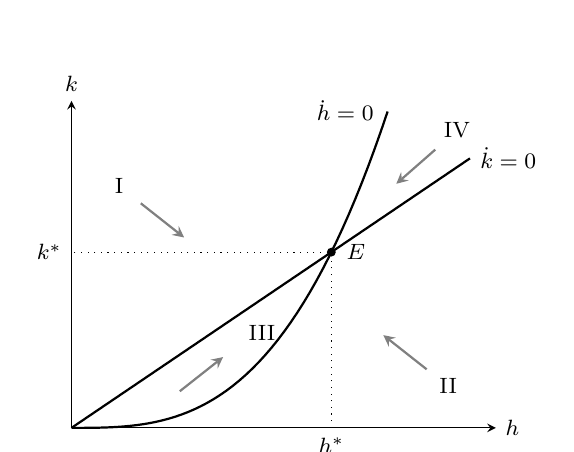
\begin{tikzpicture}[x=1.1cm,y=0.62cm,font=\footnotesize,>=stealth]
  \draw[->] (0,0) -- (4.9,0) node[right] {$h$};
  \draw[->] (0,0) -- (0,6.7) node[above] {$k$};
  \draw[thick] (0,0) -- (4.6,5.52) node[right] {$\dot k=0$};
  \draw[thick,domain=0:3.65,samples=50] plot (\x,{2/15*\x*\x*\x});
  \node[left] at (3.6,6.5) {$\dot h=0$};
  \draw[dotted] (3,0) node[below] {$h^*$} -- (3,3.6) -- (0,3.6) node[left] {$k^*$};
  \fill (3,3.6) circle (1.6pt) node[right=2pt] {$E$};
  \draw[->,thick,gray] (0.8,4.6) -- (1.3,3.9);    \node at (0.55,4.95) {I};
  \draw[->,thick,gray] (4.1,1.2) -- (3.6,1.9);    \node at (4.35,0.85) {II};
  \draw[->,thick,gray] (1.25,0.75) -- (1.75,1.45); \node at (2.2,1.95) {III};
  \draw[->,thick,gray] (4.2,5.7) -- (3.75,5.0);   \node at (4.45,6.1) {IV};
\end{tikzpicture}\\[2pt]
{\footnotesize Figure 4.8-1. The $\dot k=0$ ray, the convex $\dot h=0$ locus, and the direction of motion in
each region.}
\end{center}

\parte{c}
\passo{existence and uniqueness}{A balanced growth path is a rest point with $k,h>0$, i.e.\ a point on both loci:
$\kappa h=\lambda h^{\eta}\iff h^{\eta-1}=\kappa/\lambda$. As $\eta-1=(1-\gamma-\phi)/\gamma>0$, $h^{\eta-1}$ rises
strictly from $0$ to $\infty$, so there is exactly one positive solution,
\[ \begin{aligned}
h^*&=\Big(\frac{\kappa}{\lambda}\Big)^{\frac{\gamma}{1-\gamma-\phi}}
=\Big(\frac{c_K}{x_K}\Big)^{\frac{\gamma}{(1-\alpha)(1-\gamma-\phi)}}\Big(\frac{c_H}{x_H}\Big)^{\frac{1}{1-\gamma-\phi}},\\
k^*&=\kappa h^*=\Big(\frac{c_K}{x_K}\Big)^{\frac{1-\phi}{(1-\alpha)(1-\gamma-\phi)}}\Big(\frac{c_H}{x_H}\Big)^{\frac{1}{1-\gamma-\phi}},
\end{aligned} \]
where the exponent of $c_K/x_K$ in $k^*$ is $\frac{1}{1-\alpha}+\frac{\gamma}{(1-\alpha)(1-\gamma-\phi)}
=\frac{1-\phi}{(1-\alpha)(1-\gamma-\phi)}$. Since $\eta>1$, the ray lies above the curve for $0<h<h^*$ and below it
for $h>h^*$. The origin is the only other rest point, and the next step shows it attracts no path with $k_0,h_0>0$.}
\passo{global stability: phase diagram}{The loci cut the positive quadrant into four regions (Figure 4.8-1):
I above both ($\dot h>0$, $\dot k<0$), II below both ($\dot h<0$, $\dot k>0$), III between them with $h<h^*$
($\dot h>0$, $\dot k>0$), IV between them with $h>h^*$ ($\dot h<0$, $\dot k<0$). On the ray bounding III, $\dot k=0$
and $\dot h>0$, so the flow points right, into III; on the curve bounding III, $\dot h=0$ and $\dot k>0$, so it points
up, into III. Hence a path never leaves III, and likewise IV. In III, $k$ and $h$ rise and stay below $k^*,h^*$; in IV
they fall and stay above them; a monotone bounded path converges, and its limit must be a rest point: $E$. In I, $h$
rises and $k$ falls with $\lambda h_0^{\eta}\le\lambda h^{\eta}<k\le k_0$ and $h<k/\kappa\le k_0/\kappa$: the path either
enters III or IV or stays in I bounded away from $0$ and $\infty$, and converges to $E$ in both cases. II is symmetric
($k_0\le k<\kappa h\le\kappa h_0$ and $h>(k_0/\lambda)^{1/\eta}$). So every path with $k_0,h_0>0$ converges to $E$:
the balanced growth path exists, is unique, and is globally stable.}
\passo{local stability: Jacobian}{Using the locus conditions $c_Kk^{\alpha-1}h^{1-\alpha}=x_K$ and
$c_Hk^{\gamma}h^{\phi-1}=x_H$ at $E$,
\[ \begin{aligned}
\frac{\partial\dot k}{\partial k}&=\alpha c_Kk^{\alpha-1}h^{1-\alpha}-x_K=-(1-\alpha)x_K,&
\frac{\partial\dot k}{\partial h}&=(1-\alpha)c_Kk^{\alpha-1}h^{1-\alpha}\,\frac kh=(1-\alpha)x_K\frac{k^*}{h^*},\\
\frac{\partial\dot h}{\partial k}&=\gamma c_Hk^{\gamma}h^{\phi-1}\,\frac hk=\gamma x_H\frac{h^*}{k^*},&
\frac{\partial\dot h}{\partial h}&=\phi c_Hk^{\gamma}h^{\phi-1}-x_H=-(1-\phi)x_H.
\end{aligned} \]
Hence, since the ratios $k^*/h^*$ cancel in the determinant,
\[ \begin{aligned}
\operatorname{tr}J&=-(1-\alpha)x_K-(1-\phi)x_H<0,\\
\det J&=(1-\alpha)(1-\phi)x_Kx_H-(1-\alpha)\gamma\,x_Kx_H=(1-\alpha)(1-\gamma-\phi)\,x_Kx_H>0,\\
(\operatorname{tr}J)^2-4\det J&=\big[(1-\alpha)x_K+(1-\phi)x_H\big]^2-4(1-\alpha)(1-\phi)x_Kx_H+4(1-\alpha)\gamma\,x_Kx_H\\
&=\big[(1-\alpha)x_K-(1-\phi)x_H\big]^2+4(1-\alpha)\gamma\,x_Kx_H>0.
\end{aligned} \]
Two real negative eigenvalues: $E$ is a stable node (no oscillations), and the eigenvalue closer to zero sets the
asymptotic speed of convergence. Again $\det J>0$ is the assumption $\gamma+\phi<1$.}
\passo{growth rates on the balanced path}{With $k=k^*$ and $h=h^*$ constant, $K=k^*AL$, $H=h^*AL$ and $Y=y^*AL$ all
grow at $n+g$, and per person
\[ \frac KL=A\,k^*,\qquad\frac HL=A\,h^*,\qquad\frac YL=A\,y^*,\qquad
y^*=(1-a_K)^{\alpha}(1-a_H)^{1-\alpha}k^{*\alpha}h^{*1-\alpha}, \]
so output, physical capital and human capital per person all grow at rate $g$.}
\intuicao{$K$ helps produce $H$ and $H$ helps produce goods, hence $K$; but the feedback dies out because education
also uses $AL$, which cannot be accumulated, and $\gamma+\phi<1$ means diminishing returns to $K$ and $H$ together.
As in Solow, long-run growth per person is the exogenous $g$.}
\armadilha{The condition $\gamma+\phi<1$ does all the work. With $\gamma+\phi=1$, $\eta=1$ and the $\dot h=0$ locus is
also a ray; the two rays generically meet only at the origin, there is no rest point with $k,h>0$, and $K$ and $H$
grow at a rate that depends on $s$, $a_K$, $a_H$ and $B$: an endogenous-growth model (compare Problem 4.9).}

\parte{d}
\passo{which locus moves}{$s$ enters only $c_K$, hence only $\kappa=(c_K/x_K)^{1/(1-\alpha)}$: a permanent rise from
$s$ to $s'>s$ makes the $\dot k=0$ ray steeper and leaves the $\dot h=0$ curve unchanged. The new intersection $E'$
has higher $h^*$ and $k^*$, since both exponents of $c_K$ in part (c) are positive.}
\passo{the transition}{$k$ and $h$ are stocks, so at the date of the change, $t_0$, the economy is still at $E$, which
is on the unchanged $\dot h=0$ curve and now strictly below the new ray:
\[ \dot h(t_0)=0,\qquad\frac{\dot k(t_0)}{k^*}=\frac{s'}{s}\,c_Kk^{*\alpha-1}h^{*1-\alpha}-x_K=\Big(\frac{s'}{s}-1\Big)x_K>0. \]
The economy enters region III of the new diagram and never leaves it: $k$ and $h$ rise monotonically and converge to
$E'$, asymptotically rather than at a finite date. At first only $k$ moves (the path starts vertically); then $h$ rises
as more $K$ flows into schooling (Figure 4.8-2, left).}
\passo{output per person}{$\ln(Y/L)=\ln A+\ln y$, with $\ln y$ equal to a constant plus $\alpha\ln k+(1-\alpha)\ln h$, so
\[ \frac{d\ln(Y/L)}{dt}=g+\alpha\frac{\dot k}{k}+(1-\alpha)\frac{\dot h}{h}. \]
At $t_0$ the level does not jump ($k$ and $h$ are predetermined); its growth rate jumps from $g$ to
$g+\alpha(s'/s-1)x_K$, stays above $g$ throughout the transition ($\dot k,\dot h\ge0$, not both zero), and returns to
$g$ as $E'$ is approached. The decline need not be monotone. At $t_0$, where $\dot h=0$,
\[ \begin{aligned}
\frac{d}{dt}\frac{\dot k}{k}&=(1-\alpha)\frac{s'}{s}c_K\Big(\frac hk\Big)^{1-\alpha}\Big(\frac{\dot h}{h}-\frac{\dot k}{k}\Big)
=-(1-\alpha)\frac{s'}{s}x_K\,\frac{\dot k}{k},\\
\frac{d}{dt}\frac{\dot h}{h}&=c_Hk^{\gamma}h^{\phi-1}\Big(\gamma\frac{\dot k}{k}-(1-\phi)\frac{\dot h}{h}\Big)
=\gamma x_H\,\frac{\dot k}{k},\\
\frac{d}{dt}\Big[\alpha\frac{\dot k}{k}+(1-\alpha)\frac{\dot h}{h}\Big]_{t_0}
&=(1-\alpha)\Big(\frac{s'}{s}-1\Big)x_K\Big[\gamma x_H-\alpha\frac{s'}{s}x_K\Big],
\end{aligned} \]
so growth first accelerates when $\gamma x_H>\alpha(s'/s)x_K$: the education channel kicks in with a lag. In the
long run $\ln(Y/L)$ is higher, by the elasticity below times the change in $\ln s$, and grows at $g$ again:
\[ \frac{d\ln y^*}{d\ln s}=\alpha\frac{1-\phi}{(1-\alpha)(1-\gamma-\phi)}+(1-\alpha)\frac{\gamma}{(1-\alpha)(1-\gamma-\phi)}
=\frac{\alpha}{1-\alpha}+\frac{\gamma}{(1-\alpha)(1-\gamma-\phi)}. \]}

\begin{center}
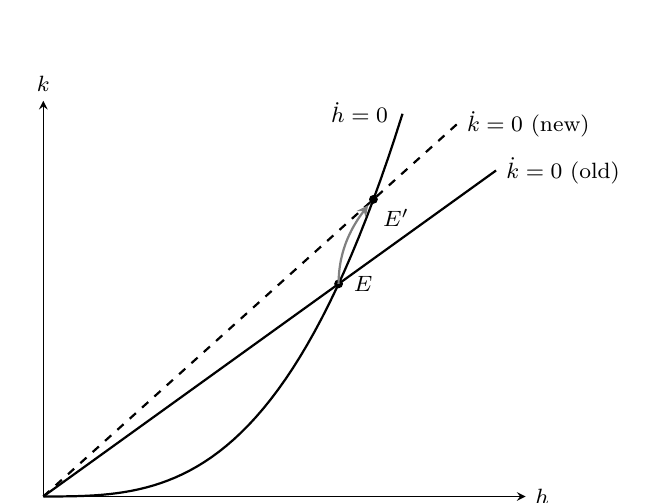
\begin{tikzpicture}[x=1.25cm,y=0.75cm,font=\footnotesize,>=stealth]
  \draw[->] (0,0) -- (4.9,0) node[right] {$h$};
  \draw[->] (0,0) -- (0,6.7) node[above] {$k$};
  \draw[thick] (0,0) -- (4.6,5.52) node[right] {$\dot k=0$ (old)};
  \draw[thick,dashed] (0,0) -- (4.2,6.3) node[right] {$\dot k=0$ (new)};
  \draw[thick,domain=0:3.65,samples=50] plot (\x,{2/15*\x*\x*\x});
  \node[left] at (3.6,6.5) {$\dot h=0$};
  \fill (3,3.6) circle (1.6pt) node[right=2pt] {$E$};
  \fill (3.354,5.031) circle (1.6pt) node[below right] {$E'$};
  \draw[->,thick,gray] (3,3.6) .. controls (3,4.2) and (3.15,4.6) .. (3.3,4.93);
\end{tikzpicture}\qquad
\begin{tikzpicture}[x=0.85cm,y=0.95cm,font=\footnotesize,>=stealth]
  \draw[->] (0,0) -- (6.8,0) node[right] {$t$};
  \draw[->] (0,0) -- (0,4.1) node[above] {$\ln(Y/L)$};
  \draw[thick] (0,0.8) -- (2,1.4);
  \draw[dashed] (2,1.4) -- (6.3,2.69);
  \draw[dotted] (2,2.3) -- (6.3,3.59);
  \draw[thick,domain=2:6.3,samples=50] plot (\x,{0.8+0.3*\x+0.9*(1-exp(-0.9*(\x-2)))});
  \draw (2,0.08) -- (2,-0.08) node[below] {$t_0$};
\end{tikzpicture}\\[2pt]
{\footnotesize Figure 4.8-2. Left: the rise in $s$ steepens the $\dot k=0$ ray; the economy moves from $E$ to $E'$
inside the new region III. Right: $\ln(Y/L)$ (solid) does not jump at $t_0$, grows faster than $g$ during the
transition, and approaches a path parallel to the old one (dashed) but higher (dotted).}
\end{center}

\intuicao{A higher $s$ raises $K$, which raises goods output directly, as in Solow, and also raises the inputs to
schooling and hence $H$: a second round of accumulation that Solow lacks. That is why the long-run elasticity
exceeds the Solow value $\alpha/(1-\alpha)$ by $\gamma/[(1-\alpha)(1-\gamma-\phi)]$. Neither round changes long-run
growth, which is pinned down by $g$: a level effect, not a growth effect.}
\armadilha{Two common slips: letting output per person jump at $t_0$ (only its growth rate jumps, because $k$ and
$h$ are stocks), and having the economy reach $E'$ at a finite date (convergence is asymptotic).}
\refbib{Romer (2012), \S4.1, pp.~151--156 (human capital in the Solow framework; the intensive-form method of
eq.~(4.7)); \S1.3--1.5, pp.~15--26 (Solow dynamics and the level effect of $s$); Problem 4.9 and Lucas (1988) for the
endogenous-growth case.}
\checado{\texttt{check-4-8-8-1.py} verifies the laws of motion from the levels, both loci and the signs off them,
$k^*$ and $h^*$, the Jacobian's trace, determinant and discriminant, growth at $g$ on the balanced path (simulated in
levels), the jump and initial slope of growth after a rise in $s$, the $s$-elasticity, monotone convergence to $E'$
and convergence from 20 random starting points. The solution manual agrees on (a)--(d); its sketch has the economy
reach $E'$ at a finite date $t_1$, whereas convergence is only asymptotic.}

% Romer (2012), Problem 8.1, p. 398 -- solution fragment for hardest-solutions.tex (statement not reproduced).
% Every key result is re-checked by hardest-parts/check-4-8-8-1.py.
\problema{Romer 8.1}{Life-cycle saving}{p.~398}{Romer \S8.1}

\noindent\textit{Notation.} $Y(t)$ is income, $W(t)$ wealth (net assets, possibly negative), $S(t)\equiv\dot W(t)$
saving and $\bar C$ the optimal consumption level. I take $Y_0>0$ and $g\ge0$ (income rising with experience); the
book does not sign $g$, and only the location of the peak of wealth in part (c) depends on it.

\parte{a}
\passo{flow constraint}{With a zero interest rate, wealth earns nothing and changes only through saving:
\[ \dot W(t)=Y(t)-C(t),\qquad W(0)=0. \]
The individual may borrow but must die without debt, $W(T)\ge0$: the continuous-time version of the requirement
behind Romer's eq.~(8.2) that any debt be repaid by the end of life.}
\passo{integrate}{Integrating from $0$ to $T$, $W(T)=W(0)+\int_0^T[Y(t)-C(t)]\,dt\ge0$, where lifetime income is
\[ \int_0^TY(t)\,dt=\int_0^R(Y_0+gt)\,dt+\int_R^T0\,dt=\Big[Y_0t+\frac g2t^2\Big]_0^R=Y_0R+\frac g2R^2. \]
So the lifetime budget constraint is
\[ \int_0^TC(t)\,dt\;\le\;Y_0R+\frac g2R^2=R\Big(Y_0+\frac{gR}{2}\Big). \]
With $r=0$ present values are plain sums: lifetime resources are the working span $R$ times average income over the
working life, $Y_0+gR/2$ (income at mid-career).}

\parte{b}
\passo{the constraint binds}{If it were slack, raising $C$ on a short interval would keep the path feasible and,
since $u'>0$, raise $U$. So the constraint holds with equality.}
\passo{first-order condition}{With multiplier $\lambda$ (Romer's eq.~(8.3) in continuous time),
\[ \begin{aligned}
\mathcal L&=\int_0^Tu(C(t))\,dt+\lambda\Big[Y_0R+\frac g2R^2-\int_0^TC(t)\,dt\Big]\\
&=\int_0^T\big[u(C(t))-\lambda C(t)\big]\,dt+\lambda\Big(Y_0R+\frac g2R^2\Big).
\end{aligned} \]
Consumption at date $t$ enters only the integrand at $t$, so $\mathcal L$ is maximized date by date:
$u'(C(t))=\lambda$ for every $t\in[0,T]$, retirement included. As $u''<0$, $u'$ is strictly decreasing, hence
one-to-one, so $C(t)=(u')^{-1}(\lambda)\equiv\bar C$ for all $t$: consumption is flat.}
\passo{the level}{Substituting the flat path into the binding constraint, $\bar C\,T=Y_0R+\frac g2R^2$, so
\[ C(t)=\bar C=\frac RT\Big(Y_0+\frac{gR}{2}\Big)=\frac1T\int_0^TY(\tau)\,d\tau\qquad\text{for all }t\in[0,T]. \]}
\passo{sufficiency}{For any path that satisfies the constraint, Jensen's inequality for the strictly concave $u$, and
then $u'>0$, give
\[ \frac1T\int_0^Tu(C(t))\,dt\;\le\;u\Big(\frac1T\int_0^TC(t)\,dt\Big)\;\le\;u(\bar C), \]
with equality only if $C(t)=\bar C$ (almost everywhere). So the flat path is the unique optimum, not merely a
stationary point.}
\intuicao{With zero interest and no discounting, a unit of consumption costs the same and is valued through the same
$u$ at every date, so diminishing marginal utility makes the individual equalize consumption across dates. $\bar C$
is permanent income, Romer's eq.~(8.5): it depends on lifetime resources, not on when income arrives, and it is the
same in retirement, when income is zero.}

\parte{c}
\passo{saving}{$S(t)=Y(t)-\bar C$: $S(t)=Y_0+gt-\bar C$ for $0\le t<R$, and $S(t)=-\bar C<0$ for $R\le t\le T$.}
\passo{working years, $0\le t\le R$}{Integrating saving from $W(0)=0$, and then using $Y_0R+\frac g2R^2=\bar CT$ at
$t=R$,
\[ W(t)=\int_0^t(Y_0+g\tau-\bar C)\,d\tau=(Y_0-\bar C)\,t+\frac g2t^2,\qquad
W(R)=Y_0R+\frac g2R^2-\bar CR=\bar C\,(T-R). \]}
\passo{retirement, $R\le t\le T$}{Wealth falls at the constant rate $\bar C$ from $W(R)$:
\[ W(t)=W(R)-\int_R^t\bar C\,d\tau=\bar C\,(T-R)-\bar C\,(t-R)=\bar C\,(T-t), \]
so $W(T)=0$: the budget is exhausted exactly at death, and in retirement wealth always equals the consumption still
to be financed.}
\passo{the hump}{On $[0,R)$, $\ddot W=g\ge0$, so $W$ is convex there and its maximum over $[0,R]$ is at an endpoint,
where $W(R)=\bar C(T-R)>0=W(0)$. Saving just before retirement is positive,
\[ S(R^-)=Y_0+gR-\bar C\;\ge\;Y_0+\frac{gR}{2}-\bar C=\Big(1-\frac RT\Big)\Big(Y_0+\frac{gR}{2}\Big)>0, \]
and on $(R,T]$ wealth falls at rate $\bar C$. So wealth peaks at retirement, with a kink there (saving drops from
$S(R^-)>0$ to $-\bar C$):
\[ \max_{0\le t\le T}W(t)=W(R)=\frac{R\,(T-R)}{T}\Big(Y_0+\frac{gR}{2}\Big). \]}
\passo{borrowing when young}{Initial saving $S(0)=Y_0-\bar C$ is negative iff $Y_0T<RY_0+\frac g2R^2$, i.e.\ iff
$gR^2>2Y_0(T-R)$: steep income growth. Wealth then falls until income reaches $\bar C$ at $t_m=(\bar C-Y_0)/g$, where
$W(t_m)=-(\bar C-Y_0)^2/g+(\bar C-Y_0)^2/(2g)=-(\bar C-Y_0)^2/(2g)<0$. Since $W(t)=t\,[\,Y_0-\bar C+\frac g2t\,]$, it is
back to zero at $\hat t=2(\bar C-Y_0)/g$, which precedes $R$ because $\bar C<Y_0+gR/2$, and it then climbs to the peak
at $R$. If $Y_0\ge\bar C$, wealth is never negative.}

\begin{center}
\begin{tikzpicture}[x=0.5cm,y=1cm,font=\footnotesize,>=stealth]
  \draw[->] (0,0) -- (10.8,0) node[right] {$t$};
  \draw[->] (0,0) -- (0,3.2) node[above] {$Y,\ C$};
  \draw[very thick] (0,0.6) -- (7,2.7);
  \draw[very thick] (7,0) -- (10,0);
  \draw[dashed] (0,1.155) -- (10,1.155) node[right] {$\bar C$};
  \draw[dotted] (7,0) node[below] {$R$} -- (7,2.7);
  \draw[dotted] (1.85,0) node[below] {$t_m$} -- (1.85,1.155);
  \node[below] at (10,0) {$T$};
  \node[left] at (0,0.6) {$Y_0$};
  \node[above left] at (5.5,2.25) {$Y(t)$};
\end{tikzpicture}\qquad
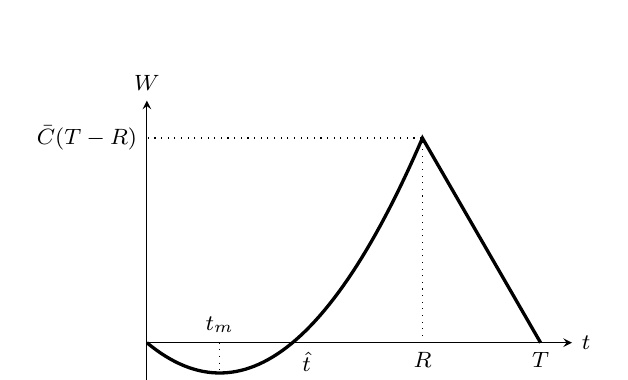
\begin{tikzpicture}[x=0.5cm,y=0.75cm,font=\footnotesize,>=stealth]
  \draw[->] (0,0) -- (10.8,0) node[right] {$t$};
  \draw[->] (0,-0.8) -- (0,4.1) node[above] {$W$};
  \draw[very thick,domain=0:7,samples=60] plot (\x,{-0.555*\x+0.15*\x*\x}) -- (10,0);
  \draw[dotted] (7,0) -- (7,3.465) -- (0,3.465) node[left] {$\bar C(T-R)$};
  \draw[dotted] (1.85,0) node[above] {$t_m$} -- (1.85,-0.513);
  \node[below] at (7,0) {$R$};
  \node[below] at (10,0) {$T$};
  \node[below right] at (3.7,0) {$\hat t$};
\end{tikzpicture}\\[2pt]
{\footnotesize Figure 8.1-1. Left: income (thick) and consumption (dashed). Right: wealth. Drawn for $Y_0=0.6$,
$g=0.3$, $R=7$, $T=10$, so $\bar C=1.155$ and $gR^2>2Y_0(T-R)$: the young borrow until $\hat t=3.7$, and wealth
peaks at $W(R)=3.465$.}
\end{center}

\intuicao{Saving is future consumption: the individual saves when income is above its lifetime average and dissaves
when it is below, so wealth is the running area between the income line and the flat consumption line. It is built
up over the working life and run down to exactly zero in retirement: the hump of Modigliani and Brumberg.}
\armadilha{The peak at $R$ uses $Y(R^-)\ge\bar C$, which $g\ge0$ guarantees. If $g<0$ and income falls to $\bar C$
before retirement, at $t_p=(Y_0-\bar C)/|g|<R$, wealth is concave on $[0,R]$ and peaks at $t_p$, while $W(T)=0$ still
holds. Nor should $W(t)\ge0$ be imposed: the book allows borrowing, and it is optimal when income grows steeply.}
\refbib{Romer (2012), \S8.1, pp.~365--368, eqs.~(8.1)--(8.6) (the discrete-time version: flat consumption, permanent
income, saving as income minus its lifetime average); Modigliani and Brumberg (1954).}
\checado{\texttt{check-4-8-8-1.py} verifies with sympy the lifetime resources, $\bar C$, both pieces of $W(t)$,
$W(R)=\bar C(T-R)$, $W(T)=0$, the borrowing condition, $t_m$, $W(t_m)$ and $\hat t<R$; numerically, that $W$ peaks at
$R$ for random $(Y_0,g,R,T)$ with $g\ge0$, that budget-neutral perturbations of the flat path lower utility (log and
CRRA $u$), and the values plotted in Figure 8.1-1. The solution manual agrees; it draws only the case $Y_0>\bar C$,
without early borrowing.}

% Romer 8.13 --- solution fragment for hardest-solutions.tex (statement not reproduced).
% Euler equations, approximations and numbers re-checked by check-8-13-8-15.py.
\problema{Romer 8.13}{Habit formation}{pp.~402--403}{Romer \S8.6}

\passo{Notation}{$\beta\equiv1/(1+\rho)$ and $u(C,Z)\equiv(C/Z)^{1-\theta}/(1-\theta)$, so lifetime utility
is $U_i=\sum_{t=1}^{T}\beta^{t}u(C_{it},Z_{it})$; the interest rate $r$ is constant and there is no
uncertainty. The derivatives used throughout are
\[
\begin{aligned}
u_C(C,Z)&=\frac1Z\Big(\frac CZ\Big)^{-\theta}=C^{-\theta}Z^{\theta-1},\qquad
u_Z(C,Z)=-\frac{C}{Z^{2}}\Big(\frac CZ\Big)^{-\theta}=-C^{1-\theta}Z^{\theta-2},\\
u_{CZ}(C,Z)&=(\theta-1)\,C^{-\theta}Z^{\theta-2},\quad\text{positive exactly when }\theta>1 .
\end{aligned}
\]}

\parte{a}
\passo{The perturbation, (i)}{Lower $C_{it}$ by $dC$ and raise $C_{i,t+1}$ by $(1+r)\,dC$. In the
present-value budget, $\sum_{t}C_{it}/(1+r)^{t}\le A_{i0}+\sum_{t}Y_{it}/(1+r)^{t}$, spending changes by
$-dC/(1+r)^{t}+(1+r)\,dC/(1+r)^{t+1}=0$: the change is feasible in either direction, so at an optimum
its first-order effect on $U_i$ is zero. The reference levels $Z_{it}=C_{t-1}^{\phi}$ and
$Z_{i,t+1}=C_{t}^{\phi}$ are aggregates that $i$ takes as given, so only the terms of $t$ and $t+1$ move:
\[
\begin{aligned}
dU_i&=-\beta^{t}C_{it}^{-\theta}Z_{it}^{\theta-1}\,dC+\beta^{t+1}C_{i,t+1}^{-\theta}Z_{i,t+1}^{\theta-1}(1+r)\,dC=0\\
\Longrightarrow\quad C_{it}^{-\theta}Z_{it}^{\theta-1}&=\frac{1+r}{1+\rho}\,C_{i,t+1}^{-\theta}Z_{i,t+1}^{\theta-1}
\qquad\text{(dividing by }\beta^{t}dC).
\end{aligned}
\]}
\passo{Euler equation, (i)}{Substitute $Z_{it}=C_{t-1}^{\phi}$ and $Z_{i,t+1}=C_{t}^{\phi}$, then divide both
sides by $C_{i,t+1}^{-\theta}C_{t-1}^{\phi(\theta-1)}$:
\[
\Big(\frac{C_{i,t+1}}{C_{it}}\Big)^{\theta}=\frac{1+r}{1+\rho}\Big(\frac{C_{t}}{C_{t-1}}\Big)^{\phi(\theta-1)}
\quad\Longrightarrow\quad
\frac{C_{i,t+1}}{C_{it}}=\Big(\frac{1+r}{1+\rho}\Big)^{1/\theta}\Big(\frac{C_{t}}{C_{t-1}}\Big)^{\phi(\theta-1)/\theta}.
\]
For $\phi=0$ this is the standard CRRA Euler equation, Romer's (8.26).}
\passo{Equilibrium, (ii)}{The representative consumer's consumption is aggregate consumption,
$C_{it}=C_t$ for all $t$, so the left side becomes $C_{t+1}/C_t$. Taking logs (exact, no approximation):
\[
\ln C_{t+1}-\ln C_{t}=a+b\,(\ln C_{t}-\ln C_{t-1}),\qquad
a\equiv\frac{\ln(1+r)-\ln(1+\rho)}{\theta}\simeq\frac{r-\rho}{\theta},\qquad
b\equiv\frac{\phi(\theta-1)}{\theta}.
\]}
\passo{$\phi>0$ and $\theta=1$}{Then $b=0$ and $\ln C_{t+1}-\ln C_t=\ln(1+r)-\ln(1+\rho)$ every period:
exactly the path without habits, so habit formation does not affect behavior. At $\theta=1$ period
utility is $\ln C_{it}-\phi\ln C_{t-1}$ and $u_C=1/C_{it}$ does not depend on $Z_{it}$: the habit
subtracts a term the individual cannot influence, which lowers the level of utility but changes no
marginal rate of substitution.}
\passo{$\phi>0$ and $\theta>1$}{Then $0<b\le(\theta-1)/\theta<1$ (because $\phi\le1$): consumption growth
is positively serially correlated. With $x_t\equiv\ln C_t-\ln C_{t-1}$, the equation $x_{t+1}=a+bx_t$ has
the fixed point and dynamics
\[
x^{*}=\frac{a}{1-b}=\frac{\ln(1+r)-\ln(1+\rho)}{\theta-\phi(\theta-1)},\qquad x_{t+1}-x^{*}=b\,(x_t-x^{*}),
\]
so a burst of growth dies out only gradually, at rate $b$ per period. Since
$1\le\theta-\phi(\theta-1)<\theta$, long-run growth also responds more to $r-\rho$ than without habits.
(For $\theta<1$, $b<0$ and growth rates alternate around $x^{*}$.)}
\intuicao{For $\theta>1$, $u_{CZ}>0$: a higher reference level raises the marginal utility of one's own
consumption (``catching up with the Joneses''). If aggregate consumption has just grown, the reference
level is higher at $t+1$ than at $t$, so marginal utility at $t+1$ is high relative to $t$ and each
consumer tilts spending toward $t+1$, i.e.\ grows faster. Everyone does the same, so past aggregate growth
feeds current growth. With $\theta=1$ the cross effect $u_{CZ}$ is zero and the habit is behaviorally
irrelevant.}

\parte{b}
\passo{Where $C_{it}$ enters, (i)}{Now $Z_{it}=C_{i,t-1}$ and $\phi=1$: $C_{it}$ is the numerator of the
period-$t$ term and the reference level of the period-$(t+1)$ term. Write
$u^{(s)}_{C}\equiv u_C(C_{is},C_{i,s-1})$ and $u^{(s)}_{Z}\equiv u_Z(C_{is},C_{i,s-1})$. The perturbation of
(a)(i) moves $C_{it}$ by $-dC$ and $C_{i,t+1}$ by $(1+r)\,dC$, so it changes utility at $t$, $t+1$ and $t+2$:
\[
\begin{aligned}
dU_i&=\beta^{t}\big[-u^{(t)}_{C}\big]dC+\beta^{t+1}\big[(1+r)\,u^{(t+1)}_{C}-u^{(t+1)}_{Z}\big]dC
+\beta^{t+2}(1+r)\,u^{(t+2)}_{Z}\,dC\\
&=-\beta^{t}M_t\,dC+\beta^{t+1}(1+r)\,M_{t+1}\,dC,\qquad M_s\equiv u^{(s)}_{C}+\beta\,u^{(s+1)}_{Z}.
\end{aligned}
\]
$M_s$ is the full marginal utility of $C_{is}$ in date-$s$ units; its second term, negative, is the
habit cost (consuming more at $s$ raises the reference level at $s+1$). At $T$ there is no such cost:
$M_T=u^{(T)}_{C}$.}
\passo{Euler equation, (i)}{Setting $dU_i=0$ gives $M_t=\frac{1+r}{1+\rho}M_{t+1}$, i.e.\ with $u_C$, $u_Z$
from the notation step,
\[
C_{it}^{-\theta}C_{i,t-1}^{\theta-1}-\frac{C_{i,t+1}^{1-\theta}C_{it}^{\theta-2}}{1+\rho}
=\frac{1+r}{1+\rho}\bigg[C_{i,t+1}^{-\theta}C_{it}^{\theta-1}-\frac{C_{i,t+2}^{1-\theta}C_{i,t+1}^{\theta-2}}{1+\rho}\bigg],
\qquad t\le T-2
\]
(for $t=T-1$ the last term is absent). Let $X_s\equiv C_{is}/C_{i,s-1}=1+g_s$. Since
$C_{is}^{-\theta}C_{i,s-1}^{\theta-1}=X_s^{1-\theta}/C_{is}$ and $C_{i,s+1}^{1-\theta}C_{is}^{\theta-2}=X_{s+1}^{1-\theta}/C_{is}$,
multiplying by $C_{i,t+1}$ and using $C_{i,t+1}/C_{it}=X_{t+1}$ gives the growth form
\[
X_{t+1}\Big[X_t^{1-\theta}-\frac{X_{t+1}^{1-\theta}}{1+\rho}\Big]=\frac{1+r}{1+\rho}\Big[X_{t+1}^{1-\theta}-\frac{X_{t+2}^{1-\theta}}{1+\rho}\Big].
\]
Only growth rates appear because $u$ is homogeneous of degree zero in $(C_{it},C_{i,t-1})$.}
\passo{Linearization, (ii)}{With $\rho=r=0$ the growth form is
$X_{t+1}\big[X_t^{1-\theta}-X_{t+1}^{1-\theta}\big]=X_{t+1}^{1-\theta}-X_{t+2}^{1-\theta}$. Replace each power by
$X_s^{1-\theta}\simeq1+(1-\theta)g_s$ (the suggested approximation with $\gamma=1-\theta$) and $X_{t+1}$ by
$1+g_{t+1}$:
\[
\begin{aligned}
\text{left side:}&\quad(1+g_{t+1})(1-\theta)(g_t-g_{t+1})=(1-\theta)(g_t-g_{t+1})
+\underbrace{(1-\theta)\,g_{t+1}(g_t-g_{t+1})}_{\text{interaction: dropped}},\\
\text{right side:}&\quad(1-\theta)(g_{t+1}-g_{t+2}).
\end{aligned}
\]
Equating the two and dividing by $-(1-\theta)$, which requires $\theta\neq1$:
\[
g_{t+2}-g_{t+1}=g_{t+1}-g_t .
\]
Keeping the interaction term instead gives $g_{t+2}-g_{t+1}=(1+g_{t+1})(g_{t+1}-g_t)$.}
\passo{Direction of the drift (exact)}{With $\rho=r=0$ the Euler equations give
$M_1=M_2=\dots=M_T\equiv\mu$, and $\mu=M_T=X_T^{1-\theta}/C_{iT}>0$. With $m_s\equiv X_s^{1-\theta}$ and
$m_{T+1}\equiv0$, $M_s=(m_s-m_{s+1})/C_{is}$ for every $s\le T$, so $m_s-m_{s+1}=\mu C_{is}$; summing over
$s=t,\dots,T$,
\[
\Big(\frac{C_{it}}{C_{i,t-1}}\Big)^{1-\theta}=\mu\sum_{s=t}^{T}C_{is}\equiv\mu R_t ,
\]
where $R_t$ is what remains to be consumed from $t$ on. For $\theta>1$, $1+g_t=(\mu R_t)^{-1/(\theta-1)}$
rises as $R_t$ falls, and to first order the constant step is $g_{t+1}-g_t\simeq\mu C_{it}/(\theta-1)>0$.
Example ($T=6$, $\theta=3$, $C_{i0}=1$, $\sum_tC_{it}=6$): consumption is U-shaped and $1+g_t$ rises from
$0.85$ to $1.60$.}
\intuicao{Internal habits make period utility a function of growth alone, so the consumer smooths growth
the way a standard consumer smooths levels. But resources move in levels: shifting a small amount from
$t$ to $t+1$ changes $(\ln X_t,\ln X_{t+1},\ln X_{t+2})$ by $(-\epsilon,+2\epsilon,-\epsilon)$, and
$\partial u/\partial\ln X=X^{1-\theta}$, so optimality sets the second difference of $X^{1-\theta}$, hence (to
first order) of $g$, to zero. Growth then changes by the same amount every period: an acceleration
persists one for one, far more persistence than external habits deliver ($b<1$). The sign comes from the
end of life: the last period carries no habit cost, so consumption is back-loaded and its growth speeds
up (in the example it first falls, lowering the habit stock).}
\armadilha{Part (b) is not part (a) with $\phi=1$: there $Z_{i,t+1}$ is taken as given, here the $u_Z$ term is
internalized. And the division by $1-\theta$ is not innocuous. At $\theta=1$ with $\rho=0$ lifetime utility
telescopes to $\ln C_{iT}-\ln C_{i0}$ and the Euler equation reads $0=0$; for $\theta<1$ letting $C_{it}\to0$
for one period makes $(C_{i,t+1}/C_{it})^{1-\theta}$, and so $U_i$, unbounded. With $\rho=0$, as in (ii), the
problem has a maximum only for $\theta>1$.}
\refbib{Romer \S8.4, pp.~380--381, eqs.~(8.24)--(8.26) (CRRA Euler equation by the same perturbation);
\S8.6, p.~390, n.~14 (habit-formation literature); ch.~7, p.~358 (habits as a source of sluggish
consumption).}
\checado{\texttt{check-8-13-8-15.py} differentiates the perturbed utility symbolically and confirms, at
random points, the (a)(i) Euler ratio and the (b)(i) Euler equation and its growth form; checks $b=0$ at
$\theta=1$, $0<b<1$ for $\theta>1$ and $x^{*}$; series-expands the (b) condition to first order; and solves
the $T=6$ example numerically, confirming $M_t$ constant, $X_t^{1-\theta}/R_t$ constant and rising growth.
The Romer solution manual agrees with (a) and (b); it asserts without proof that growth increases over
time, which the exact step establishes for $\theta>1$.}

% Romer 8.15 --- solution fragment for hardest-solutions.tex (statement not reproduced).
% Closed forms, the naive = sophisticated result and the CRRA numbers re-checked by check-8-13-8-15.py.
\problema{Romer 8.15}{Time-inconsistent preferences}{pp.~403--404}{Romer \S8.6}

\passo{Environment}{With $r=0$ the only constraint is $c_1+c_2+c_3=W$. The date-1 self weights
$(\ln c_1,\ln c_2,\ln c_3)$ by $(1,\delta,\delta)$ and the date-2 self weights $(\ln c_2,\ln c_3)$ by $(1,\delta)$:
quasi-hyperbolic ($\beta$--$\delta$) discounting with short-run factor $\delta$ and long-run factor $1$. Every
future date is discounted by $\delta$ relative to ``now'', but two future dates are not discounted
relative to each other. Every objective below is a sum of strictly concave functions of the choice
variables on a convex set, so first-order conditions identify the maxima.}

\parte{a}
\passo{(i) Commitment}{Substitute $c_3=W-c_1-c_2$ into the date-1 objective and differentiate with
respect to $c_1$ and $c_2$:
\[
\frac{1}{c_1}-\frac{\delta}{W-c_1-c_2}=0,\qquad\frac{\delta}{c_2}-\frac{\delta}{W-c_1-c_2}=0 .
\]
The second condition gives $c_2=c_3$; the first gives $c_3=\delta c_1$. The budget then reads
$c_1+2\delta c_1=W$:
\[
c_1^{C}=\frac{W}{1+2\delta},\qquad c_2^{C}=c_3^{C}=\frac{\delta W}{1+2\delta}.
\]}
\passo{The date-2 self's rule}{At date 2 the remaining wealth is $W_2\equiv W-c_1$ and the date-2 self
maximizes $\ln c_2+\delta\ln(W_2-c_2)$: $1/c_2=\delta/(W_2-c_2)$, so $W_2-c_2=\delta c_2$ and
\[
c_2=\frac{W_2}{1+\delta},\qquad c_3=\frac{\delta W_2}{1+\delta}.
\]
The rule is proportional to wealth, with date-2 share $s^{*}\equiv1/(1+\delta)>1/2$.}
\passo{(ii) Naivete}{The naif expects to follow the date-1 plan, so it solves the commitment problem and
picks $c_1^{N}=c_1^{C}$. Then $W_2=W-c_1^{N}=2\delta W/(1+2\delta)$ and the date-2 rule gives
\[
c_1^{N}=\frac{W}{1+2\delta},\qquad c_2^{N}=\frac{2\delta}{1+\delta}\cdot\frac{W}{1+2\delta},\qquad
c_3^{N}=\frac{2\delta^{2}}{1+\delta}\cdot\frac{W}{1+2\delta}.
\]}
\passo{(iii) Sophistication}{The sophisticate substitutes the date-2 rule, with $W_2=W-c_1$, into its
date-1 objective:
\[
\ln c_1+\delta\ln\frac{W-c_1}{1+\delta}+\delta\ln\frac{\delta(W-c_1)}{1+\delta}
=\ln c_1+2\delta\ln(W-c_1)+\delta\ln\frac{\delta}{(1+\delta)^{2}} .
\]
The first-order condition $1/c_1=2\delta/(W-c_1)$ gives $W-c_1=2\delta c_1$, so $c_1^{S}=W/(1+2\delta)=c_1^{N}$;
the same date-2 rule then gives $c_2^{S}=c_2^{N}$ and $c_3^{S}=c_3^{N}$.}

\parte{b}
\passo{(i) In what sense preferences are time-inconsistent}{Seen from date 1, $c_2$ and $c_3$ carry the
same weight, so the plan is $c_3/c_2=1$. At date 2 the same person, with no new information, sets
$c_3/c_2=\delta<1$; comparing (a)(ii) with (a)(i),
\[
\frac{c_2^{N}}{c_2^{C}}=\frac{2}{1+\delta}>1,\qquad\frac{c_3^{N}}{c_3^{C}}=\frac{2\delta}{1+\delta}<1 .
\]
The marginal rate of substitution between $c_2$ and $c_3$ depends on the date at which it is evaluated,
not only on the dates at which consumption occurs, so the plan that is optimal at date 1 is no longer
optimal at date 2 and is abandoned. (With exponential weights $(1,\delta,\delta^2)$ and $(1,\delta)$ the ratio
of the weights on $c_3$ and $c_2$ is $\delta$ at both dates, and plans are kept.) The date-1 self loses
from the revision, since $c_1$ is the same in both cases:
\[
U_1^{C}-U_1^{N}=\delta\ln\frac{c_2^{C}c_3^{C}}{c_2^{N}c_3^{N}}=\delta\ln\frac{(1+\delta)^{2}}{4\delta}>0,
\]
because $(1+\delta)^2-4\delta=(1-\delta)^2>0$; it would pay for a commitment device, such as the illiquid
saving Romer mentions on p.~398.}
\passo{(ii) Why sophistication changes nothing}{Let the date-2 split be any rule proportional to wealth,
$c_2=sW_2$ and $c_3=(1-s)W_2$, with $s\in(0,1)$ independent of $W_2$. The date-1 objective is then
\[
\ln c_1+\delta\ln[s(W-c_1)]+\delta\ln[(1-s)(W-c_1)]=\ln c_1+2\delta\ln(W-c_1)+\delta\ln[s(1-s)],
\]
so $s$ enters only through an additive constant, and the first-order condition $1/c_1=2\delta/(W-c_1)$
does not contain $s$: $c_1=W/(1+2\delta)$ for every $s$. The naif uses $s=1/2$, the sophisticate
$s=s^{*}$; both choose the same $c_1$, after which the same date-2 self chooses $c_2$ and $c_3$.
Equivalently, the marginal value of saving at date 1 is
\[
\delta\Big[\frac{1}{c_2}\frac{\partial c_2}{\partial W_2}+\frac{1}{c_3}\frac{\partial c_3}{\partial W_2}\Big]
=\delta\Big[\frac{s}{sW_2}+\frac{1-s}{(1-s)W_2}\Big]=\frac{2\delta}{W_2},
\]
independent of $s$.}
\intuicao{The sophisticate knows that a unit saved will go mostly to $c_2$, where its marginal utility is
low, and less to $c_3$, where it is high. With log utility, marginal utility times consumption is one,
so each share times its marginal utility equals $1/W_2$ and the two effects cancel exactly. Put
differently, the future self's misallocation works like a lower return on saving, and with log utility
the income and substitution effects of a change in the return offset each other.}
\passo{What changes with CRRA utility}{Replace $\ln c$ by $u(c)=c^{1-\sigma}/(1-\sigma)$, $\sigma>0$,
$\sigma\neq1$, in both objectives. Commitment: $c_1^{-\sigma}=\delta c_2^{-\sigma}=\delta c_3^{-\sigma}$, so
$c_2=c_3=\delta^{1/\sigma}c_1$ and $c_1^{C}=c_1^{N}=W/(1+2\delta^{1/\sigma})$. Date 2: $c_2^{-\sigma}=\delta c_3^{-\sigma}$
gives $c_3=\delta^{1/\sigma}c_2$, again a proportional rule, with $s^{*}=1/(1+\delta^{1/\sigma})$. For any share
$s$, $u(sW_2)=s^{1-\sigma}u(W_2)$, so the date-1 problem and its first-order condition are
\[
\begin{aligned}
&\max_{c_1}\;u(c_1)+\delta A(s)\,u(W-c_1),\qquad A(s)\equiv s^{1-\sigma}+(1-s)^{1-\sigma},\\
&c_1^{-\sigma}=\delta A(s)\,(W-c_1)^{-\sigma}\;\Longrightarrow\;c_1=\frac{W}{1+[\delta A(s)]^{1/\sigma}} .
\end{aligned}
\]
Now $s$ scales the marginal value of saving instead of shifting a constant. The naif's $s=1/2$ gives
$A=2^{\sigma}$ and returns the commitment $c_1$. $A$ is symmetric about $1/2$ with
$A''(s)=-\sigma(1-\sigma)[s^{-\sigma-1}+(1-s)^{-\sigma-1}]$, and $s^{*}\neq1/2$. For $\sigma<1$, $A$ is concave
with its maximum at $1/2$, so $A(s^{*})<2^{\sigma}$ and $c_1^{S}>c_1^{N}$: the substitution effect dominates
and the sophisticate saves less. For $\sigma>1$, $A$ is convex with its minimum at $1/2$, so
$c_1^{S}<c_1^{N}$: the income effect dominates and it saves more to offset its future self's
overspending. With $\delta=1/2$: $\sigma=2$ gives $c_1^{S}=0.4106W<c_1^{N}=0.4142W$, and $\sigma=1/2$ gives
$c_1^{S}=0.6897W>c_1^{N}=0.6667W$.}
\armadilha{Naivete and commitment share $c_1$ by construction, so the inconsistency shows up only in
$(c_2,c_3)$; comparing first-period choices cannot reveal it. And the equivalence of naive and
sophisticated choices is a property of log utility, not of the $\beta$--$\delta$ structure: the date-2 rule
is proportional to wealth for every CRRA utility, but only under log does the share drop out of the
marginal value of saving.}
\refbib{Romer \S8.6, pp.~397--398 (time-inconsistent preferences; Laibson, 1997); \S8.4, pp.~381--383
(income and substitution effects of the interest rate).}
\checado{\texttt{check-8-13-8-15.py} solves the commitment, date-2, naive and sophisticated problems
symbolically, verifies that the cross derivative $\partial^2/\partial c_1\partial s$ of the date-1 objective
under an arbitrary share $s$ is zero, checks $U_1^{C}-U_1^{N}=\delta\ln[(1+\delta)^2/(4\delta)]>0$, and for
$\sigma\in\{2,1/2\}$ re-derives $s^{*}$, $c_1^{N}$ and $c_1^{S}$ by numerical maximization, matching the
closed forms and the printed numbers. The Romer solution manual agrees; its (b)(ii) gives the same two
offsetting effects and states, without derivation, that with other utility functions either ordering is
possible, which the CRRA step makes precise.}

% Romer 10.16 --- solution fragment for hardest-solutions.tex (statement not reproduced).
% Numbers and identities re-checked by check-10-16-2-9.py.
\problema{Romer 10.16}{Search efficiency with a general matching function}{p.~512}{Romer \S10.7}

\passo{Environment}{The static economy of eqs.~(10.71)--(10.75): a given pool of $U$ unemployed
workers; $V$ vacancies, each created at cost $c$; $E=M(U,V)$ matches, each producing $y$; wage
$w=\phi y$; no income for the unemployed. The wage is a transfer between matched parties, so welfare
is $W(V)=M(U,V)\,y-cV$. Only the matching function changes. ``Well-behaved'' is taken to mean: $M$ is
smooth, $M_V>0$, $M_{VV}<0$, $M(U,0)=0$ and $M\le V$ (a filling probability cannot exceed one); neither
Cobb--Douglas form nor constant returns is assumed. Because $U$ is fixed, the only margin is $V$.
Define the job-filling probability $q$ and the elasticity of matches with respect to vacancies $\eta$:
\[
q(V)\equiv\frac{M(U,V)}{V},\qquad
\eta(V)\equiv\frac{V\,M_V(U,V)}{M(U,V)}.
\]}

\passo{The elasticity lies in $(0,1)$}{Strict concavity puts the tangent line at $V$ above the
function at $0$: $M(U,0)<M(U,V)+M_V(U,V)\,(0-V)$. With $M(U,0)=0$ this reads $V M_V<M$, so
$\eta(V)<1$; and $M_V>0$ gives $\eta(V)>0$. Differentiating $q$,
\[
q'(V)=\frac{V M_V-M}{V^2}=-\frac{q(V)}{V}\,\bigl[1-\eta(V)\bigr]<0 .
\]}

\passo{Decentralized equilibrium}{A vacancy is filled with probability $q(V)$, and a filled job
leaves the firm $y-w=(1-\phi)y$. The expected value of opening a vacancy is $q(V)(1-\phi)y-c$; free
entry drives it to zero (eq.~(10.71) with a general $M$):
\[
\frac{M(U,V^{EQ})}{V^{EQ}}\,(1-\phi)\,y=c. \qquad\text{(F)}
\]
The left side is strictly decreasing in $V$ because $q'<0$, so (F) has at most one root; it exists
($V^{EQ}>0$) by assumption, hence it is unique.}

\passo{Planner}{The planner chooses $V$ to maximize $W(V)=M(U,V)\,y-cV$:
\[
W'(V)=M_V(U,V)\,y-c,\qquad W''(V)=M_{VV}(U,V)\,y<0 .
\]
$W$ is strictly concave, so the first-order condition (eq.~(10.74) with a general $M$)
\[
M_V(U,V^{*})\,y=c \qquad\text{(P)}
\]
is necessary and sufficient, and $V^*$ is unique.}

\passo{The wedge between (P) and (F)}{By the definition of $\eta$, $M_V=\eta(V)\,M/V=\eta(V)\,q(V)$
at every $V$, so $W'(V)=\eta(V)\,q(V)\,y-c$. At $V=V^{EQ}$, replace $c$ using (F):
\[
W'(V^{EQ})=\eta(V^{EQ})\,q(V^{EQ})\,y-(1-\phi)\,q(V^{EQ})\,y
=q(V^{EQ})\,y\,\bigl[\eta(V^{EQ})-(1-\phi)\bigr].
\]}

\passo{Efficiency condition}{($\Leftarrow$) If $\eta(V^{EQ})=1-\phi$, the bracket is zero, so
$W'(V^{EQ})=0$: $V^{EQ}$ solves (P), whose only root is $V^*$; hence $V^{EQ}=V^*$.
($\Rightarrow$) If $V^{EQ}=V^*$, then $W'(V^{EQ})=0$; since $q(V^{EQ})\,y>0$, the bracket vanishes:
$\eta(V^{EQ})=1-\phi$. Therefore
\[
V^{EQ}=V^{*}\quad\Longleftrightarrow\quad
\frac{V\,M_V(U,V)}{M(U,V)}\bigg|_{V=V^{EQ}}=1-\phi .
\]
The answer is \textbf{yes}: the condition survives without Cobb--Douglas form or constant returns, with
one qualification --- the elasticity is evaluated at the equilibrium allocation. Evaluating it at $V^*$
instead is equivalent: if $\eta(V^*)=1-\phi$, then by (P)
$q(V^*)(1-\phi)y=\eta(V^*)\,q(V^*)\,y=M_V(U,V^*)\,y=c$, so $V^*$ solves (F), and since the root of (F) is
unique, $V^{EQ}=V^*$.}

\passo{Direction of the inefficiency}{$W'$ is strictly decreasing and $W'(V^*)=0$. If
$\eta(V^{EQ})<1-\phi$, then $W'(V^{EQ})<0$, so $V^{EQ}>V^*$: too many vacancies. If
$\eta(V^{EQ})>1-\phi$, then $W'(V^{EQ})>0$ and $V^{EQ}<V^*$: too few. This is Romer's result for
$\gamma\lessgtr 1-\phi$, with $\gamma$ replaced by the elasticity at the equilibrium point.}

\passo{What a general $M$ changes}{Under Cobb--Douglas, $\eta\equiv\gamma$ at every point, so the
condition restricts parameters only. In general $\eta$ varies with $(U,V)$ and $V^{EQ}$ depends on
$\phi$, $y$, $c$ and $U$, so the condition restricts the equilibrium point. Example, neither
Cobb--Douglas nor constant-returns: $M=UV/(1+U+V)$, which meets every assumption above. Here
$M_V=U(1+U)/(1+U+V)^2$, $q=U/(1+U+V)$ and $\eta=(1+U)/(1+U+V)$, so
\[
\begin{gathered}
\text{(F)}:\ 1+U+V^{EQ}=\frac{(1-\phi)\,yU}{c},\qquad
\text{(P)}:\ \bigl(1+U+V^{*}\bigr)^2=\frac{yU(1+U)}{c},\\
V^{EQ}=V^*\iff 1-\phi=\Bigl[\frac{c\,(1+U)}{yU}\Bigr]^{1/2}.
\end{gathered}
\]
The last equivalence squares (F) and compares it with (P). With $U=1$, $y=8$, $c=1$: $\phi=\tfrac12$
gives $V^{EQ}=V^*=2$ and $\eta(V^{EQ})=\tfrac12=1-\phi$; $\phi=\tfrac14$ gives $V^{EQ}=4>V^*=2$, with
$\eta(V^{EQ})=\tfrac13<\tfrac34$. The efficient share moves with $c/y$ and with the size of the
unemployment pool, so no fixed bargaining rule is efficient for all fundamentals.}

\intuicao{Split the gap between the social and the private value of a marginal vacancy:
\[
\underbrace{M_V\,y}_{\text{social}}-\underbrace{q\,(1-\phi)\,y}_{\text{private}}
=\underbrace{\phi\,y\,M_V}_{\text{gain to workers}}
-\underbrace{(1-\phi)\,y\,(q-M_V)}_{\text{congestion on other firms}} .
\]
The entrant expects $q$ matches, but total matches rise only by $M_V=\eta q$: the other
$q-M_V=(1-\eta)q$ are taken from other vacancies, each worth $(1-\phi)y$ to its owner, while each new
match hands $\phi y$ to a worker. The two externalities cancel iff $M_V=(1-\phi)q$, that is,
$\eta=1-\phi$. The accounting never uses the functional form; it only has to balance where entry stops.}

\armadilha{(i) Treating $\eta=1-\phi$ as a restriction on parameters: with a general $M$ it must hold at
$V^{EQ}$, which itself moves with $\phi$; a point $\hat V\neq V^{EQ}$ with $\eta(\hat V)=1-\phi$ proves
nothing. (ii) Thinking constant returns are needed: $U$ is fixed here, so only the $V$-elasticity
enters; in the dynamic model constant returns matter only because they make $\eta$ a function of
tightness $V/U$ alone.}

\refbib{Romer (2012), \S10.7, eqs.~(10.71)--(10.75) and the welfare discussion, pp.~497--498;
Hosios (1990); Rogerson, Shimer and Wright (2005).}

\checado{\texttt{check-10-16-2-9.py} verifies with sympy, for an arbitrary $M(U,V)$, the identity
$W'(V)-[q(1-\phi)y-c]=q\,y\,[\eta-(1-\phi)]$ and the externality split; for $M=UV/(1+U+V)$ it checks
$\eta$, $M_{VV}<0$ and non-constant returns, then solves (F) and (P) by root-finding with $U=1$, $y=8$,
$c=1$: $\phi=\tfrac12$ gives $V^{EQ}=V^*=2$; $\phi=\tfrac14$ gives $V^{EQ}=4>V^*$; $\phi=0.6$ gives
$V^{EQ}=1.2<V^*$; at $U=3$ the efficient $\phi\approx0.59$, not $\tfrac12$. The solution manual also
answers yes; it does not state where $\eta$ is evaluated or the direction of the inefficiency.}

% Romer 2.9 --- solution fragment for hardest-solutions.tex (statement not reproduced).
% Identities, the closed-form path and the numerical integration are re-checked by check-10-16-2-9.py.
\problema{Romer 2.9}{A closed-form solution of the Ramsey model}{p.~95}{Romer \S2.2--2.6}

\passo{Model and maintained assumptions}{Romer's Ramsey model in units of effective labor: no
depreciation, $f(k)=k^\alpha$ with $0<\alpha<1$, household utility weighted by $L(t)/H$, and
$\beta\equiv\rho-n-(1-\theta)g>0$ (eq.~(2.2)); take $n+g>0$. The equations of motion are
\[
\frac{\dot c}{c}=\frac{f'(k)-\rho-\theta g}{\theta}\quad(2.24),\qquad
\dot k=f(k)-c-(n+g)k\quad(2.25).
\]
With $\theta=\alpha$ and $f'(k)=\alpha k^{\alpha-1}$, (2.24) becomes
\[
\frac{\dot c}{c}=\frac{\alpha k^{\alpha-1}-\rho-\alpha g}{\alpha}
=k^{\alpha-1}-\frac{\rho+\alpha g}{\alpha}. \qquad(\star)
\]}

\parte{a}
\passo{$\dot c=0$}{With $c>0$, $(\star)$ vanishes iff $\alpha k^{*\,\alpha-1}=\rho+\alpha g$, i.e.\
$k^{*\,1-\alpha}=\alpha/(\rho+\alpha g)$. Raising both sides to the power $1/(1-\alpha)$:
\[
k^*=\Bigl(\frac{\alpha}{\rho+\alpha g}\Bigr)^{1/(1-\alpha)} .
\]}

\parte{b}
\passo{$\dot k=0$}{(2.25) at $k^*$ gives $c^*=k^{*\alpha}-(n+g)k^*=k^*\bigl[k^{*\,\alpha-1}-(n+g)\bigr]$.
Substitute $k^{*\,\alpha-1}=(\rho+\alpha g)/\alpha$ from (a):
\[
c^*=k^*\Bigl[\frac{\rho+\alpha g}{\alpha}-n-g\Bigr]=\frac{\rho-\alpha n}{\alpha}\,k^*
=\frac{\rho-\alpha n}{\alpha}\Bigl(\frac{\alpha}{\rho+\alpha g}\Bigr)^{1/(1-\alpha)} .
\]
It is positive: expanding, $\beta+(1-\alpha)(n+g)=\rho-n-(1-\alpha)g+(1-\alpha)n+(1-\alpha)g=\rho-\alpha n$,
so $\rho-\alpha n>0$. Define $x^*\equiv c^*/k^*=(\rho-\alpha n)/\alpha$.}

\parte{c}
\passo{$\dot z$}{Since $y=k^\alpha$, $z=k/y=k^{1-\alpha}$ and $k^{\alpha-1}=1/z$. By the chain rule and (2.25),
\[
\begin{aligned}
\dot z&=(1-\alpha)k^{-\alpha}\dot k=(1-\alpha)k^{-\alpha}\bigl[k^\alpha-c-(n+g)k\bigr]
=(1-\alpha)\Bigl[1-\frac{c}{k}\,k^{1-\alpha}-(n+g)\,k^{1-\alpha}\Bigr]\\
&=(1-\alpha)\bigl[1-(x+n+g)\,z\bigr].
\end{aligned}
\]}
\passo{$\dot x/x$}{$\ln x=\ln c-\ln k$, so $\dot x/x=\dot c/c-\dot k/k$. From $(\star)$,
$\dot c/c=1/z-(\rho+\alpha g)/\alpha$; from (2.25), $\dot k/k=k^{\alpha-1}-c/k-(n+g)=1/z-x-n-g$. Hence
\[
\frac{\dot x}{x}=\frac1z-\frac{\rho}{\alpha}-g-\frac1z+x+n+g=x-\frac{\rho-\alpha n}{\alpha}=x-x^* .
\]
The $1/z$ terms cancel only because $\theta=\alpha$: the marginal product raises consumption growth by
$f'(k)/\theta=(\alpha/\theta)k^{\alpha-1}$, the average product raises capital growth by $k^{\alpha-1}$.}

\parte{d}
\passo{The conjecture is the saddle path}{If $x$ is constant, $\dot x=x(x-x^*)=0$ with $x>0$ forces
$x(t)=x^*$ for all $t$: the saddle path is the ray $c=x^*k$. No other path is admissible. Let $u\equiv1/x$;
then $\dot u=-\dot x/x^2=-(x-x^*)/x=x^*u-1$, so $u(t)=1/x^*+[u(0)-1/x^*]\,e^{x^*t}$. If $x(0)>x^*$, $u$
reaches $0$ at $T=\ln[x(0)/(x(0)-x^*)]/x^*$: $c/k\to\infty$ in finite time, so $k$ is driven to zero
while $c>0$ --- the paths above the saddle path that Romer rules out in \S2.3 (at $k=0$, $c$ would have
to jump to zero, violating (2.24)). If $x(0)<x^*$, $u\to\infty$ and $x\to0$; by (c), $z\to1/(n+g)$, so
$f'(k)=\alpha/z\to\alpha(n+g)<n+g$ and $e^{-R(s)}e^{(n+g)s}k(s)\to\infty$: households would not exhaust
lifetime wealth, the paths below the saddle path ruled out in \S2.3 using (2.15).}
\passo{(i) Path of $z$}{With $x=x^*$, use $x^*+n+g=(\rho-\alpha n+\alpha n+\alpha g)/\alpha
=(\rho+\alpha g)/\alpha=1/z^*$, where $z^*\equiv k^{*\,1-\alpha}=\alpha/(\rho+\alpha g)$. Then
\[
\dot z=(1-\alpha)\Bigl[1-\frac{z}{z^*}\Bigr]=-\lambda\,(z-z^*),\qquad
\lambda\equiv\frac{1-\alpha}{z^*}=\frac{(1-\alpha)(\rho+\alpha g)}{\alpha}.
\]
Since $\tfrac{d}{dt}\bigl[e^{\lambda t}(z-z^*)\bigr]=e^{\lambda t}\bigl[\dot z+\lambda(z-z^*)\bigr]=0$, we have
$e^{\lambda t}[z(t)-z^*]=z(0)-z^*$, that is,
\[
z(t)=z^*+\bigl[z(0)-z^*\bigr]e^{-\lambda t}.
\]}
\passo{(ii) Path of $y$}{$y=k^\alpha=(k^{1-\alpha})^{\alpha/(1-\alpha)}=z^{\alpha/(1-\alpha)}$ and
$z(0)=k(0)^{1-\alpha}$, so
\[
y(t)=\Bigl\{k^{*\,1-\alpha}+\bigl[k(0)^{1-\alpha}-k^{*\,1-\alpha}\bigr]e^{-\lambda t}\Bigr\}^{\alpha/(1-\alpha)},
\qquad k^{*\,1-\alpha}=\frac{\alpha}{\rho+\alpha g},
\]
with $k(t)=z(t)^{1/(1-\alpha)}$, $c(t)=x^*k(t)$ and $y^*=z^{*\,\alpha/(1-\alpha)}=k^{*\alpha}$.}
\passo{Speed of convergence}{Let $a\equiv\alpha/(1-\alpha)$, so $y=z^a$, and use $|y-y^*|$ so the log
is defined on either side of $y^*$. With $\dot y=a z^{a-1}\dot z=-\lambda a z^{a-1}(z-z^*)$,
\[
\frac{d\ln|y-y^*|}{dt}=\frac{\dot y}{y-y^*}=-\lambda\,\psi(z),\qquad
\psi(z)\equiv\frac{a z^{a-1}(z-z^*)}{z^a-z^{*a}} .
\]
As $z\to z^*$, $(z^a-z^{*a})/(z-z^*)\to a z^{*\,a-1}$, so $\psi\to1$: the asymptotic speed is $\lambda$.
But $\psi$ is constant only if $a=1$, i.e.\ $\alpha=\theta=\tfrac12$ (then $y=z$ and the speed is exactly
$\lambda$). For $\alpha<\tfrac12$, $z^a$ is concave: below the balanced growth path ($z<z^*$) the slope
$a z^{a-1}$ exceeds the chord slope $(z^{*a}-z^a)/(z^*-z)$, so $\psi>1$; above it, $\psi<1$. With
$\alpha=\tfrac13$, $a=\tfrac12$ and $\psi=\tfrac12 z^{-1/2}(z^{1/2}+z^{*1/2})=\tfrac12(1+y^*/y)$: an economy
starting at $y=y^*/2$ converges at $1.5\lambda$ and slows to $\lambda$. So the answer is \textbf{no}: the
rate is constant for $z$, not for $y$.}
\passo{Link to the linearization of \S2.6}{With $\theta=\alpha$, $f''(k^*)c^*/\theta
=(\alpha-1)k^{*\,\alpha-1}x^*=-\lambda x^*$ (using $k^{*\,\alpha-1}=1/z^*$ and $(1-\alpha)/z^*=\lambda$).
Then (2.36) at $\mu=-\lambda$ reads $\lambda^2+\beta\lambda-\lambda x^*=\lambda(\lambda+\beta-x^*)$, and
\[
\alpha(\lambda+\beta-x^*)=(1-\alpha)(\rho+\alpha g)+\alpha\rho-\alpha n-\alpha(1-\alpha)g-\rho+\alpha n=0 .
\]
So Romer's negative root $\mu_1$ in (2.39) equals $-\lambda$ exactly, and the linearized saddle path
($\dot{\tilde k}=\beta\tilde k-\tilde c=\mu_1\tilde k$, i.e.\ $\tilde c=(\beta+\lambda)\tilde k=x^*\tilde k$)
is the exact ray $c=x^*k$. The linearization is exact for $z$; its error for $y$ comes only from the
curvature of $y=z^a$.}

\parte{e}
\passo{Equation (2.25)}{On the conjectured path $k=z^{1/(1-\alpha)}$, so
$\dot k=\frac{1}{1-\alpha}z^{\alpha/(1-\alpha)}\dot z=z^{\alpha/(1-\alpha)}\bigl(1-z/z^*\bigr)
=z^{\alpha/(1-\alpha)}-z^{1/(1-\alpha)}/z^*$. The right side of (2.25), using $c=x^*k$ and
$x^*+n+g=1/z^*$, is $k^\alpha-(x^*+n+g)k=z^{\alpha/(1-\alpha)}-z^{1/(1-\alpha)}/z^*$. They coincide.}
\passo{Equation (2.24)}{With $x^*$ constant, $\dot c/c=\dot k/k=z^{\alpha/(1-\alpha)-1/(1-\alpha)}-1/z^*
=1/z-1/z^*=k^{\alpha-1}-(\rho+\alpha g)/\alpha$, which is $(\star)$, i.e.\ (2.24) with $\theta=\alpha$.}
\passo{Conclusion}{Both equations of motion hold at every $t$, the path starts at the given $k(0)$, and
$(k,c)\to(k^*,c^*)$, so $f'(k)\to\rho+\theta g$ and $e^{-R(s)}e^{(n+g)s}k(s)$ eventually falls at rate
$\beta>0$: (2.15) holds with equality. \textbf{Yes} --- the conjecture is the equilibrium path, and by
the argument in (d) it is the only one.}

\intuicao{Consumption growth loads on the average product $y/k$ with weight $\alpha/\theta$ (because
$f'(k)=\alpha y/k$); capital growth loads on it with weight $1$. With $\theta=\alpha$ the weights coincide,
so $c$ and $k$ grow at the same rate whenever $c/k=x^*$: households consume a fixed fraction $x^*$ of
their capital. The capital-output ratio then obeys a linear equation and converges at the constant rate
$\lambda$; output inherits a varying rate because $y=z^{\alpha/(1-\alpha)}$ is curved.}

\armadilha{Adding depreciation (Romer's chapter~2 has none); writing $\rho+g$ instead of $\rho+\theta g$
in the Euler equation; and reading the constant rate of $z$ as a constant rate for $y$.}

\refbib{Romer (2012), eqs.~(2.2), (2.15), (2.24)--(2.25), (2.36)--(2.39); \S2.3 (saddle path) and
\S2.6 (speed of adjustment); Smith (2006).}

\checado{\texttt{check-10-16-2-9.py} re-derives $\dot z$ and $\dot x/x$ from (2.24)--(2.25) with sympy;
checks $k^*$, $c^*$, the $u=1/x$ solution and blow-up time, that the closed-form path satisfies
(2.24)--(2.25) identically, and that (2.39) with $\theta=\alpha$ gives $\mu_1=-\lambda$ and saddle slope
$x^*$; integrates (2.24)--(2.25) numerically from $c(0)=x^*k(0)$ ($\alpha=\theta=\tfrac13$, $\rho=0.04$,
$n=0.01$, $g=0.02$, $k(0)=k^*/2$) and matches $z(t)$ to the closed form; and confirms
$\psi=\tfrac12(1+y^*/y)>1$ for $\alpha=\tfrac13$ and $\psi\equiv1$ for $\alpha=\tfrac12$. The solution
manual agrees on (a)--(e); it calls the speed ``clearly not constant'' without the $\alpha=\tfrac12$
exception, and leaves $x=x^*$ a conjecture checked only through (e).}

% Romer 2.12 (with 2.10-2.11 as far as needed). Checked by check-2-12-11-1.py; the figures plot its paths.
\problema{Romer 2.12}{Temporary taxes on investment income}{p.~96}{Romer \S2.6--2.7, problems 2.10--2.11}
Notation of Romer ch.~2: $k$ and $c$ per unit of effective labor, no depreciation, CRRA utility with
coefficient $\theta$, and $\rho-n-(1-\theta)g>0$. Investment income is taxed at $\tau(t)\in\{0,\tau\}$,
$0<\tau<1$, and the revenue is rebated lump-sum (the setting of 2.10). Problems 2.10--2.11 are solved
only as far as 2.12 needs them.

\passo{The two systems of dynamics (2.10a)}{A household holding $k_h$ has the flow budget
$\dot k_h=(1-\tau(t))f'(k)k_h+w+T-c-(n+g)k_h$, with wage $w=f(k)-kf'(k)$ and a transfer
$T=\tau(t)f'(k)k$ that does not depend on its own $k_h$. Its Euler equation is Romer's (2.20) with the
after-tax return $r(t)=(1-\tau(t))f'(k(t))$; imposing $k_h=k$ in the budget,
\[ \begin{aligned}
\frac{\dot c}{c}&=\frac{(1-\tau(t))f'(k)-\rho-\theta g}{\theta},\\
\dot k&=(1-\tau)f'(k)k+\bigl[f(k)-kf'(k)\bigr]+\tau f'(k)k-c-(n+g)k=f(k)-c-(n+g)k.
\end{aligned} \]
The tax drops out of the resource constraint, so the $\dot k=0$ locus $c=\bar c(k)\equiv f(k)-(n+g)k$
does not move. The $\dot c=0$ locus moves from $f'(k^*)=\rho+\theta g$ to
$f'(k_\tau)=(\rho+\theta g)/(1-\tau)>\rho+\theta g$; as $f''<0$, $k_\tau<k^*$: the vertical line shifts
left. Call N the untaxed system (steady state $E=(k^*,c^*)$, saddle path $S_N$) and T the taxed one
($E_\tau=(k_\tau,c_\tau)$, saddle path $S_T$). Since $\rho+\theta g>n+g$, $f'(k^*)>n+g=f'(k_{GR})$, so
$k^*<k_{GR}$, $\bar c$ is increasing on $(0,k^*]$ and $c_\tau<c^*$.}

\passo{Regions and traps}{Under T, $\dot c<0$ iff $k>k_\tau$, and $\dot k<0$ iff $c>\bar c(k)$. Let
\[ A=\{k>k_\tau,\ c>\bar c(k)\},\qquad B=\{k>k_\tau,\ c<\bar c(k)\},\qquad C=\{k<k_\tau,\ c>\bar c(k)\}: \]
in $A$ both variables fall; in $B$, $c$ falls and $k$ rises; in $C$, $c$ rises and $k$ falls.
$B$ and $C$ are traps. In $B$, $k$ rises, so
$k_\tau$ is never reached, and on the locus the motion is straight down, back into $B$. In $C$, $k$
falls, and $c$ rises while $\bar c(k)$ falls with $k$, so neither boundary is ever reached. $A_N$, $B_N$,
$C_N$ are the same regions under N, with $k^*$ in place of $k_\tau$. Along $S_N$, $c$ and $k$ move
together toward $E$, so $S_N$ is increasing; it lies strictly below $\bar c$ for $k<k^*$ (there
$\dot k>0$) and above $c^*$ for $k>k^*$.}

\passo{What can jump, and when (2.11b)}{$k$ is a stock with finite $\dot k$, so it is continuous. For $c$,
Romer's (2.18) gives $\theta\ln c(t)=\ln B-\ln\lambda-\beta t+R(t)-(n+g)t$, with
$R(t)=\int_0^t r(s)\,ds$. $R$ is continuous even at the dates where $r$ jumps (the start or end of the
tax), so for a given $\lambda$ the path of $c$ is continuous. The multiplier $\lambda$, the marginal
utility of initial wealth, is set when the plan is made and changes only when news arrives. Here the
only news date is $0$, so $c$ can jump at $0$ and nowhere else. In words: a foreseen upward jump at
$t'$ would let the household gain a first-order amount of utility by moving consumption from just
after $t'$ to just before it, at a negligible cost in interest.}

\passo{Where the economy must be when the last regime starts}{After the last change of regime, N
governs forever and Romer's \S2.3 argument applies: above $S_N$, $k$ hits zero in finite time and $c$
would then have to jump down (ruled out above); below $S_N$, $c\to0$ while $k$ rises past $k_{GR}$, and
households hold capital whose present value never vanishes, violating the transversality condition.
So at the date of the last change the economy must be on $S_N$. Neither $k$ nor $c$ jumps at that
foreseen date, so the dynamics of the preceding regime must carry it onto $S_N$ exactly then ($S_N$ is
not invariant under T, so arriving early does not help). With a permanent tax the target is $S_T$
instead: in 2.10(b) $c$ jumps at $0$ straight onto $S_T$; in 2.11 it jumps by less at $0$, drifts
northwest under N and reaches $S_T$ exactly at $t_1$.}

\parte{a}
\passo{Regimes}{T on $[0,t_1)$, N from $t_1$ on, news only at $0$. So $c$ jumps at $0$ to some $c_0$,
both variables are continuous at $t_1$, and the T-trajectory from $(k^*,c_0)$ must be on $S_N$
exactly at $t_1$.}
\passo{The jump is upward}{If $c_0<c^*$, the point $(k^*,c_0)$ is in $B$; if $c_0=c^*$, it is on the
locus with $\dot k=0>\dot c$ and enters $B$ at once. Either way the path is trapped in $B$, with
$k(t)>k^*$ and $c(t)<c^*$ for all $t>0$, while $S_N$ lies above $c^*$ wherever $k>k^*$: $S_N$ is never
reached. Hence $c_0>c^*$.}
\passo{Dynamics while the tax is in force}{$(k^*,c_0)$ is in $A$, so $c$ and $k$ both start to fall.
If the path stayed in $A$ until $t_1$, it would be above $\bar c$ at some $k<k^*$, where $S_N$ lies
below $\bar c$; if it entered the trap $C$, it would stay above $\bar c$ for good. So it must cross the
$\dot k=0$ locus into $B$ at some $t_m<t_1$, at $k_m\in(k_\tau,k^*)$; from then on $c$ keeps falling
while $k$ rises. At $t_1$, $c(t_1)<c(t_m)=\bar c(k_m)<\bar c(k^*)=c^*$, and since $S_N$ is increasing,
$k(t_1)<k^*$. A path starting on or above $S_T$ cannot cross $S_T$ and never enters $B$, so $c_0$ lies
strictly between $c^*$ and the height of $S_T$ at $k^*$: the jump is smaller than under the permanent
tax of 2.10(b). By continuity some $c_0$ in that interval arrives on $S_N$ exactly at $t_1$ (the
arrival time tends to $0$ as $c_0\downarrow c^*$ and to infinity as $c_0$ approaches $S_T$).}
\passo{After the tax is removed}{The economy rides $S_N$ up to $E$: $c$ and $k$ both rise. At $t_1$ the
$\dot c=0$ line jumps back from $k_\tau$ to $k^*$, so $\dot c$ switches from negative to positive (a
kinked trough in $c$), while $\dot k=f(k)-c-(n+g)k$ is continuous ($k$ is smooth). In sum: $c$ jumps up
at $0$, falls throughout the tax period to below $c^*$ and then rises back to $c^*$; $k$ falls to a
minimum at $t_m<t_1$, is already rising when the tax ends, and returns to $k^*$.}

\begin{center}
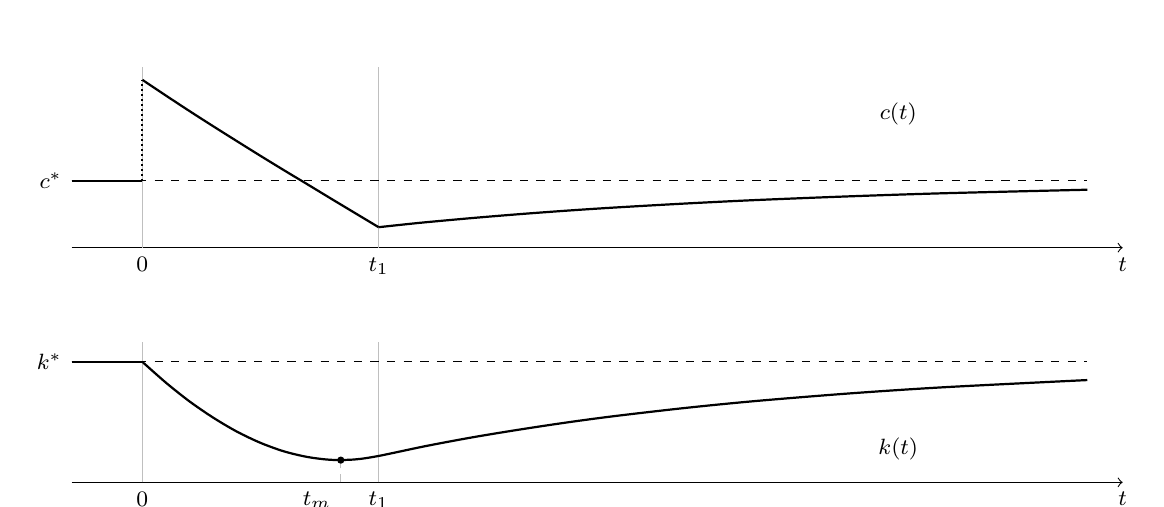
\begin{tikzpicture}[x=0.3cm,font=\footnotesize]
\begin{scope}[y=0.17cm]
  \draw[->] (-3,-5) -- (41.5,-5) node[below]{$t$};
  \foreach \x/\l in {0/0,10/t_1} \draw[gray!50] (\x,-5) node[below,black]{$\l$} -- (\x,8.5);
  \draw[dashed] (-3,0) node[left]{$c^*$} -- (40,0);
  \draw[thick] (-3,0) -- (0,0);
  \draw[thick,densely dotted] (0,0) -- (0,7.54);
  \draw[thick] plot[smooth] coordinates {(0,7.54) (1,6.36) (2,5.20) (3,4.07) (4,2.96) (5,1.86) (6,0.78) (7,-0.28) (8,-1.35) (9,-2.41) (10,-3.47)};
  \draw[thick] plot[smooth] coordinates {(10,-3.47) (11,-3.28) (12,-3.10) (14,-2.78) (16,-2.49) (18,-2.23) (20,-2.00) (23,-1.70) (26,-1.44) (30,-1.16) (34,-0.93) (40,-0.67)};
  \node at (32,5) {$c(t)$};
\end{scope}
\begin{scope}[yshift=-2.3cm,y=0.17cm]
  \draw[->] (-3,-9) -- (41.5,-9) node[below]{$t$};
  \foreach \x/\l in {0/0,10/t_1} \draw[gray!50] (\x,-9) node[below,black]{$\l$} -- (\x,1.5);
  \draw[gray!50,densely dashed] (8.4,-9) node[below left,black]{$t_m$} -- (8.4,-7.34);
  \draw[dashed] (-3,0) node[left]{$k^*$} -- (40,0);
  \draw[thick] (-3,0) -- (0,0);
  \draw[thick] plot[smooth] coordinates {(0,0.00) (1,-1.56) (2,-2.96) (3,-4.17) (4,-5.21) (5,-6.05) (6,-6.69) (7,-7.11) (8,-7.32) (9,-7.29) (10,-7.03) (12,-6.29) (14,-5.63) (16,-5.05) (18,-4.52) (20,-4.05) (23,-3.44) (26,-2.92) (30,-2.35) (34,-1.89) (40,-1.36)};
  \fill (8.4,-7.34) circle (1.3pt);
  \node at (32,-6.5) {$k(t)$};
\end{scope}
\end{tikzpicture}\par
{\footnotesize (a): tax on $[0,10)$. Simulated paths ($f=k^{1/3}$, $\rho=0.04$, $\theta=2$, $n=0.01$,
$g=0.02$, $\tau=0.3$), plotted as $100\ln(c/c^*)$ and $100\ln(k/k^*)$; dotted: the jump at $0$.}
\end{center}

\intuicao{While the tax is in force the after-tax return is below $\rho+\theta g$, so the Euler equation
makes consumption fall; once it is lifted, capital is scarce ($k<k^*$), the return exceeds
$\rho+\theta g$ and consumption grows back. With no long-run change and no jump allowed at $t_1$,
consumption must start the tax period above $c^*$ and end it below: households consume more and invest
less while saving is penalized, and start rebuilding capital before $t_1$ because they know the high
untaxed return is coming. The revenue is rebated, so the resource constraint is unchanged and the
whole effect works through the after-tax return; it is weaker than for a permanent tax because saving
is penalized only for a while.}

\parte{b}
\passo{Regimes}{N on $[0,t_1)$, T on $[t_1,t_2)$, N from $t_2$ on, news only at $0$. So $c$ jumps only
at $0$, is continuous at $t_1$ and $t_2$, and the economy must reach $S_N$ exactly at $t_2$. Before $t_1$
the untaxed Euler equation governs $c$: the $\dot c=0$ line is still at $k^*$.}
\passo{The jump is upward}{If $c_0=c^*$, the economy rests at $E$ until $t_1$ and then faces the
situation ruled out in (a). If $c_0<c^*$, $(k^*,c_0)$ is in $B_N$, a trap of N, so at $t_1$ it has
$k>k^*$ and $c<c^*$: it is then in the trap $B$ of T and never reaches $S_N$, which lies above $c^*$
for $k>k^*$. Hence $c_0>c^*$.}
\passo{Between the announcement and $t_1$}{At $(k^*,c_0)$, $\dot c=0$ and $\dot k=c^*-c_0<0$; once
$k<k^*$, $\dot c>0$. The path is in $C_N$, a trap of N: $c$ rises and $k$ falls until $t_1$. This is an
explosive path of N (on its own it would drive $k$ to zero); it is the equilibrium path only because
the regime changes before it explodes.}
\passo{While the tax is in force}{At $t_1$ the $\dot c=0$ line jumps to $k_\tau$ while $(k,c)$ is
continuous. If $k(t_1)\le k_\tau$, the point would be in (or enter) $C$, a trap above $\bar c$, and
$S_N$ would never be reached. So $k(t_1)>k_\tau$, the point is in $A$, and the argument of (a) applies
with $t_2$ in place of $t_1$: $c$ falls throughout $(t_1,t_2)$; $k$ keeps falling until the path
crosses the locus at $t_m\in(t_1,t_2)$ and rises afterwards; at $t_2$ the economy is on $S_N$ with
$c<c^*$ and $k<k^*$.}
\passo{After the tax ends}{The economy rides $S_N$ up to $E$. In sum: $c$ jumps up at $0$, rises until
$t_1$ (a kinked peak, as $\dot c$ turns negative), falls during the tax period to below $c^*$ (a kinked
trough at $t_2$) and returns to $c^*$; $k$ falls from $0$ to a minimum at $t_m\in(t_1,t_2)$ and then
rises smoothly back to $k^*$.}

\begin{center}
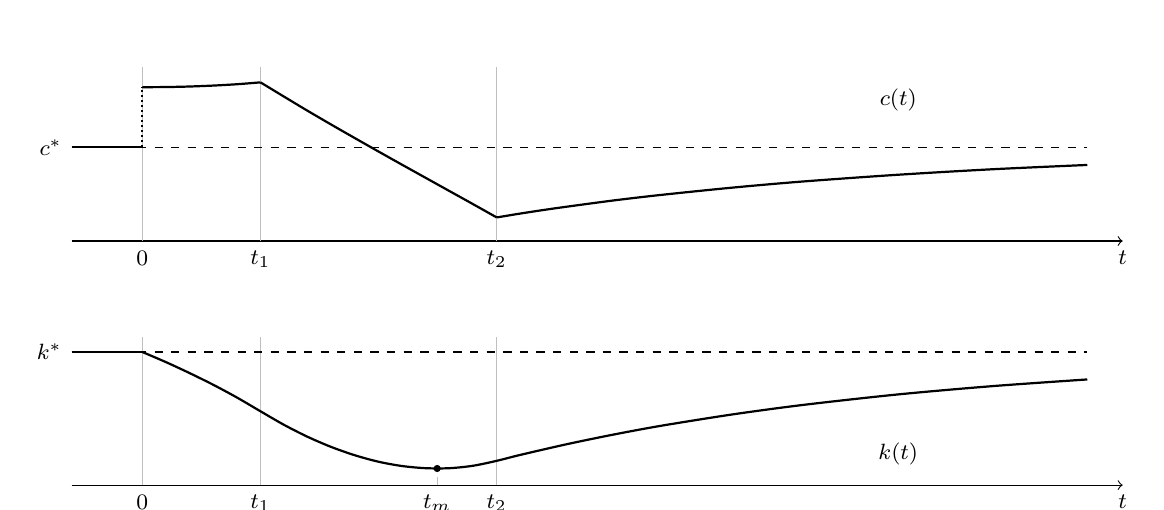
\begin{tikzpicture}[x=0.3cm,font=\footnotesize]
\begin{scope}[y=0.17cm]
  \draw[->] (-3,-7) -- (41.5,-7) node[below]{$t$};
  \foreach \x/\l in {0/0,5/t_1,15/t_2} \draw[gray!50] (\x,-7) node[below,black]{$\l$} -- (\x,6);
  \draw[dashed] (-3,0) node[left]{$c^*$} -- (40,0);
  \draw[thick] (-3,0) -- (0,0);
  \draw[thick,densely dotted] (0,0) -- (0,4.49);
  \draw[thick] plot[smooth] coordinates {(0,4.49) (1,4.50) (2,4.54) (3,4.61) (4,4.71) (5,4.85)};
  \draw[thick] plot[smooth] coordinates {(5,4.85) (6,3.78) (7,2.72) (8,1.69) (9,0.68) (10,-0.32) (11,-1.31) (12,-2.29) (13,-3.27) (14,-4.25) (15,-5.24)};
  \draw[thick] plot[smooth] coordinates {(15,-5.24) (16,-4.95) (17,-4.68) (18,-4.43) (20,-3.96) (22,-3.55) (25,-3.01) (28,-2.55) (32,-2.05) (36,-1.64) (40,-1.32)};
  \node at (32,3.5) {$c(t)$};
\end{scope}
\begin{scope}[yshift=-2.6cm,y=0.13cm]
  \draw[->] (-3,-13) -- (41.5,-13) node[below]{$t$};
  \foreach \x/\l in {0/0,5/t_1,15/t_2} \draw[gray!50] (\x,-13) node[below,black]{$\l$} -- (\x,1.5);
  \draw[gray!50,densely dashed] (12.48,-13) node[below,black]{$t_m$} -- (12.48,-11.38);
  \draw[dashed] (-3,0) node[left]{$k^*$} -- (40,0);
  \draw[thick] (-3,0) -- (0,0);
  \draw[thick] plot[smooth] coordinates {(0,0.00) (1,-0.99) (2,-2.06) (3,-3.20) (4,-4.44) (5,-5.79) (6,-7.12) (7,-8.29) (8,-9.28) (9,-10.09) (10,-10.72) (11,-11.14) (12,-11.35) (13,-11.35) (14,-11.11) (15,-10.63) (16,-10.05) (18,-8.99) (20,-8.04) (22,-7.19) (25,-6.09) (28,-5.16) (32,-4.14) (36,-3.33) (40,-2.68)};
  \fill (12.48,-11.38) circle (1.3pt);
  \node at (32,-10) {$k(t)$};
\end{scope}
\end{tikzpicture}\par
{\footnotesize (b): tax on $[5,15)$, announced at $0$. Same calibration and units as in (a).}
\end{center}

\intuicao{Anticipated policy moves the economy before it is implemented. Households know that saving will
be poorly rewarded during $[t_1,t_2)$, so consumption must fall over that window (Euler). Since $c$
cannot jump at $t_1$, the high level from which it falls must be built up beforehand, and under the
untaxed Euler equation consumption grows only if $f'(k)>\rho+\theta g$, i.e.\ only if capital is
already below $k^*$. So the economy starts to decumulate at the announcement, and consumption is
front-loaded relative to the tax period.}

\armadilha{(i) Letting $c$ jump when the tax starts or ends: both dates are known at $0$. (ii) In (a),
sending the economy to $S_T$: that answers the permanent tax of 2.10(b); with a temporary tax the target
is $S_N$ at $t_1$, and the economy is never on $S_T$. (iii) Claiming that $k$ falls during the whole
tax period: the landing point on $S_N$ lies below the $\dot k=0$ locus, so $k$ is already rising when
the tax ends. (iv) Shifting the $\dot k=0$ locus: it stays put because the revenue is rebated; it would
shift down if the revenue financed government purchases (2.10f).}

\refbib{Romer (2012), \S2.2--2.3 (eqs.~(2.17)--(2.18), (2.24)--(2.25), the saddle path), \S2.6 (an
unanticipated change: jump onto the new saddle path), \S2.7 (temporary versus permanent changes);
problems 2.10--2.11, pp.~95--96.}
\checado{\texttt{check-2-12-11-1.py} confirms symbolically that the rebate leaves $\dot k$ unchanged,
then simulates the calibrated economy by shooting $c_0$ for 2.10(b), 2.11 and both parts here, and
asserts every claim above: $c^*<c_0$, with jumps $100\ln(c_0/c^*)$ of $11.3$ (2.10b), $7.5$ (a) and
$4.5$ (b); the monotonicity of $c$ on each interval and the sign switch of $\dot c$ at the policy dates;
the minimum of $k$ at $t_m\approx8.4<t_1=10$ in (a) and at $t_m\approx12.5\in(5,15)$ in (b); and arrival
on $S_N$ (traced separately by backward integration) exactly at the last switch, with $c<c^*$, $k<k^*$.
Romer's solution manual (pp.~2-18--2-19) reaches the same answer for both parts.}

% Romer 11.1. Checked by check-2-12-11-1.py (sympy).
\problema{Romer 11.1}{The forward-looking Cagan model}{p.~576}{Romer \S11.1}
Money demand as given in the problem, with $b>0$ and $c$ a constant: real balances $m_t-p_t$ fall when
expected inflation $E_tp_{t+1}-p_t$ rises, because with output and the real rate fixed, higher expected
inflation raises the nominal rate (the Fisher identity (11.3)) and with it the cost of holding money.
Write $\phi\equiv b/(1+b)\in(0,1)$, so that $1-\phi=1/(1+b)$. Nothing below uses more than the
linearity of $E_t$ and the law of iterated projections, so $E_t$ can be read as perfect foresight
($E_tx_{t+i}=x_{t+i}$) throughout.

\parte{a}
\passo{Collect the terms in $p_t$}{Expanding the right side, $m_t-p_t=c-bE_tp_{t+1}+bp_t$, so
$(1+b)p_t=m_t-c+bE_tp_{t+1}$ and
\[ p_t=\frac{1}{1+b}(m_t-c)+\frac{b}{1+b}\,E_tp_{t+1}=(1-\phi)(m_t-c)+\phi E_tp_{t+1}. \]
Today's price level is a weighted average of $m_t-c$ (the price level that would clear the market with
zero expected inflation) and the price level expected for tomorrow.}

\parte{b}
\passo{Shift one period and take expectations}{(a) holds at every date, so
$p_{t+1}=(1-\phi)(m_{t+1}-c)+\phi E_{t+1}p_{t+2}$. Applying $E_t$, which is linear,
\[ E_tp_{t+1}=(1-\phi)(E_tm_{t+1}-c)+\phi E_t\bigl[E_{t+1}p_{t+2}\bigr]
=(1-\phi)(E_tm_{t+1}-c)+\phi E_tp_{t+2}, \]
by the law of iterated projections: everything known at $t$ is still known at $t+1$, so
$E_t[E_{t+1}x]=E_tx$; today's forecast of tomorrow's forecast is today's forecast (a predictable revision
would mean today's forecast is not rational).}

\parte{c}
\passo{Iterate}{Substituting (b) into (a) gives
$p_t=(1-\phi)(m_t-c)+\phi(1-\phi)(E_tm_{t+1}-c)+\phi^2E_tp_{t+2}$. By induction, for every $n\ge1$,
\[ p_t=(1-\phi)\sum_{i=0}^{n-1}\phi^i\,(E_tm_{t+i}-c)+\phi^n E_tp_{t+n},\qquad E_tm_t=m_t. \]
For $n=1$ this is (a). If it holds for $n$, apply (a) at $t+n$ and take $E_t$ with the law of iterated
projections, $E_tp_{t+n}=(1-\phi)(E_tm_{t+n}-c)+\phi E_tp_{t+n+1}$; substituting turns the last term
into $(1-\phi)\phi^n(E_tm_{t+n}-c)+\phi^{n+1}E_tp_{t+n+1}$, which is the formula for $n+1$.}
\passo{Impose no bubbles}{The problem's condition is $\lim_{n\to\infty}\phi^nE_tp_{t+n}=0$. Letting
$n\to\infty$ and using $(1-\phi)\sum_{i\ge0}\phi^i=(1-\phi)/(1-\phi)=1$ (valid as $0<\phi<1$),
\[ p_t=-c+\sum_{i=0}^{\infty}\frac{b^i}{(1+b)^{i+1}}\,E_tm_{t+i}, \]
provided expected money grows by less than the factor $1/\phi=(1+b)/b$ per period. The weights are
positive and sum to one: $p_t+c$ is a weighted average of current and expected future money stocks.}
\passo{Why the condition is needed}{(a) alone does not pin down $p_t$. If $p^F_t$ is the solution above
and $B_t$ satisfies $E_tB_{t+1}=B_t/\phi$, then $p^F_t+B_t$ also satisfies (a): the extra terms are $B_t$
on the left and $\phi E_tB_{t+1}=B_t$ on the right. Such a bubble is expected to grow at rate $1/b$ per
period, pushing expected inflation up and real balances down without end (Romer's footnote~1,
p.~516). Since $\phi^nE_tB_{t+n}=B_t$ for all $n$, the no-bubbles condition says exactly $B_t=0$.}

\parte{d}
\passo{The chain of expectations}{From (c), $\partial p_t/\partial E_tm_{t+i}=b^i/(1+b)^{i+1}>0$. The
mechanism runs backward in time. Money-market equilibrium at $t+i$ makes the expected price level
$E_tp_{t+i}$ higher. Then expected inflation from $t+i-1$ to $t+i$ is higher, so the nominal rate at
$t+i-1$ is higher and real money demand at $t+i-1$ is lower; with $m_{t+i-1}$ unchanged, $p_{t+i-1}$
must rise to shrink real balances. That raises expected inflation from $t+i-2$ to $t+i-1$, and so on
back to $t$: higher expected inflation from $t$ to $t+1$ lowers the demand for real balances today, and
since $m_t$ is given, only a higher $p_t$ clears the money market. Each step back passes on the fraction
$\phi=b/(1+b)$ of the effect, so it decays geometrically with the horizon, and more slowly the more
interest-elastic money demand is (larger $b$). If the whole expected path of money rises by one unit,
$p_t$ rises by one unit, since the weights sum to one.}
\intuicao{The price level behaves like an asset price: it is the present value of current and future
fundamentals (the money stocks), discounted at rate $1/b$, since $1/(1+1/b)=\phi$. News about future
money moves today's price level before any money is printed, just as news about future dividends moves
today's share price.}

\parte{e}
\passo{Substitute the path}{With $E_tm_{t+i}=m_t+gi$ in the formula of (c),
\[ p_t=-c+(1-\phi)\sum_{i=0}^{\infty}\phi^i(m_t+gi)=m_t-c+g\,(1-\phi)S,\qquad
S\equiv\sum_{i=0}^{\infty}i\,\phi^i. \]}
\passo{Evaluate the series}{The $i=0$ term of $S$ is zero, so $S=\sum_{j\ge1}j\phi^j$, while
$\phi S=\sum_{i\ge0}i\phi^{i+1}=\sum_{j\ge1}(j-1)\phi^j$. Subtracting,
$S-\phi S=\sum_{j\ge1}\phi^j=\phi/(1-\phi)$, so $S=\phi/(1-\phi)^2$ and
$(1-\phi)S=\phi/(1-\phi)=\dfrac{b/(1+b)}{1/(1+b)}=b$. Hence
\[ p_t=m_t-c+bg. \]}
\passo{Check}{The same formula one period ahead gives $E_tp_{t+1}=m_t+g-c+bg$, so expected inflation is
$E_tp_{t+1}-p_t=g$ and $m_t-p_t=c-bg=c-b(E_tp_{t+1}-p_t)$: money demand holds. The no-bubbles condition
holds too, since $\phi^n(m_t+gn-c+bg)\to0$.}
\passo{Effect of $g$}{$\partial p_t/\partial g=b>0$. With $m_t$ given, faster expected money growth
raises expected inflation one for one, raises the nominal rate (the Fisher effect) and lowers the demand
for real balances by $b$ per unit of $g$; the money market clears today only if $p_t$ jumps up by
$b\,\Delta g$, and real balances $m_t-p_t=c-bg$ fall. This is the discrete-time counterpart of Romer's
Figure~11.2: when a higher money growth rate becomes known, the price level jumps although the money
stock does not.}
\intuicao{What sets today's price level is the expected path of money, not just its current stock.
Run in reverse, the same result says that a credible disinflation (a fall in $g$) lowers $p_t$ on
impact unless $m_t$ jumps up by $b\,|\Delta g|$, which is why the ends of hyperinflations come with
bursts of money growth while prices stabilize (Romer, pp.~517--518).}

\armadilha{(i) Shifting (a) forward but keeping $E_t$ inside: the shifted equation holds with
$E_{t+1}p_{t+2}$, and only the law of iterated projections turns $E_t[E_{t+1}p_{t+2}]$ into
$E_tp_{t+2}$. (ii) Mishandling the constant: each term carries $-(1-\phi)\phi^i c$, and these add up to
exactly $-c$. (iii) Reading $\partial p_t/\partial g=b$ as an effect that arrives with the extra money:
it is immediate, through expected inflation and money demand, with $m_t$ unchanged.}

\refbib{Romer (2012), \S11.1, pp.~514--518 (eq.~(11.3), Figure~11.2, footnote~1 on bubble paths); the
no-bubbles condition parallels problem 8.8.}
\checado{\texttt{check-2-12-11-1.py} re-derives (a) with sympy and verifies: the iterated formula of
(c) over eight forward substitutions; the weights $b^i/(1+b)^{i+1}$ and their unit sum; the series
$\sum_i i\phi^i=\phi/(1-\phi)^2$; the closed form $p_t=m_t-c+bg$, by symbolic summation and by a
3{,}000-term numerical sum; that it clears the money market and satisfies the no-bubbles condition;
$\partial p_t/\partial g=b$; and that adding a bubble with $E_tB_{t+1}=B_t/\phi$ preserves (a). Romer's
solution manual (pp.~11-1--11-2) agrees: $p_t=m_t-c+bg$ and $\partial p_t/\partial g=b$.}

% Romer 11.22 --- solution fragment for hardest-solutions.tex (statement not reproduced).
% Law of motion, steady states, stability signs and simulations re-checked by check-11-22-6-16.py.
\problema{Romer 11.22}{Cagan with adaptive expectations}{p.~583}{Romer \S11.9}

\passo{Environment}{Notation of \S11.9: $m\equiv M/P$ (real balances), $g_M\equiv\dot M/M$,
$\pi\equiv\dot P/P$; $S^{\mathrm{MAX}}$ is the largest seignorage that can be collected in a steady
state. In our words, the two assumptions are: real balances always equal Cagan's demand evaluated at
\emph{expected} inflation, $m=Ce^{-b\pi^e}$ ($C,b>0$); expectations move toward actual inflation at
speed $\beta$, $\dot\pi^e=\beta(\pi-\pi^e)$, with $0<\beta<1/b$. As in the text, real purchases $G$
are financed entirely by money creation, so $S(t)=G$ at every date.}

\parte{a}
\passo{Real balances inherit the motion of expectations}{Taking logs, $\ln m(t)=\ln C-b\pi^e(t)$;
differentiating with respect to time,
\[ \frac{\dot m(t)}{m(t)}=-b\,\dot\pi^e(t). \tag{1} \]}

\passo{The financing constraint}{Seignorage is $S=\dot M/P=(\dot M/M)(M/P)=g_M m$, so $S=G$ gives
$g_M=G/m$. Since $m=M/P$, $\dot m/m=g_M-\pi$; hence, using (1),
\[ \pi(t)=g_M(t)-\frac{\dot m(t)}{m(t)}=\frac{G}{m(t)}+b\,\dot\pi^e(t). \tag{2} \]
At a given instant $\pi^e(t)$ is predetermined, and so is $m(t)=Ce^{-b\pi^e(t)}$; the two unknowns
are $\pi(t)$ and $\dot\pi^e(t)$, linked by (2) and by the adaptive rule.}

\passo{Solve the two equations}{Substituting (2) into $\dot\pi^e=\beta(\pi-\pi^e)$,
\[ \dot\pi^e=\beta\Big[\frac{G}{m}+b\,\dot\pi^e-\pi^e\Big]
\quad\Longrightarrow\quad (1-b\beta)\,\dot\pi^e=\beta\Big[\frac{G}{m}-\pi^e\Big]. \]
Because $b\beta<1$ we can divide by $1-b\beta>0$; substituting $m=Ce^{-b\pi^e}$ then gives
\[ \begin{aligned}
\dot\pi^e(t)&=\frac{\beta}{1-b\beta}\;\frac{G-\pi^e(t)\,m(t)}{m(t)}\\
&=\frac{\beta}{1-b\beta}\Big[\frac{G}{C}\,e^{b\pi^e(t)}-\pi^e(t)\Big]\equiv\Phi\big(\pi^e(t)\big).
\end{aligned} \tag{3} \]}

\passo{Actual inflation}{From the adaptive rule, $\pi=\pi^e+\dot\pi^e/\beta$; with (3),
\[ \pi(t)=\pi^e(t)+\frac{G/m(t)-\pi^e(t)}{1-b\beta}=\frac{G/m(t)-b\beta\,\pi^e(t)}{1-b\beta}. \tag{4} \]}

\passo{The same law of motion as (11.75)}{Write $\pi^e=(\ln C-\ln m)/b$ and combine (1) with (3):
\[ \frac{\dot m}{m}=-b\,\dot\pi^e=\frac{b\beta}{1-b\beta}\;\frac{1}{m}\Big[\frac{\ln C-\ln m}{b}\,m-G\Big], \]
which is exactly (11.75). The two models are one model: in \S11.9 define $x\equiv(\ln C-\ln m)/b$,
the inflation rate that would make current holdings desired; then (11.71) reads $\dot x=\beta(\pi-x)$,
an adaptive rule for $x$. Figures 11.9--11.10 are thus the phase diagrams of this problem in
$(\ln m,\dot m/m)$ space; since $(\ln m,\dot m/m)=(\ln C-b\pi^e,\,-b\dot\pi^e)$, the diagrams in
$(\pi^e,\dot\pi^e)$ below are those figures rotated by $180^\circ$ and rescaled.}

\armadilha{The book asks for $\dot\pi^e$ ``as a function of $\pi(t)$''. Read literally, the adaptive
rule already is one; the analogue of (11.75) gives the motion of the state variable in terms of the
state alone, which is (3) (the solution manual reads it the same way). $\pi$ cannot serve as the
argument: by (4), $d\pi/d\pi^e=b\,(g_M-\beta)/(1-b\beta)$ changes sign where $g_M=\beta$, so two values
of $\pi^e$ map into the same $\pi$. Dropping the term $b\dot\pi^e$ in (2), i.e.\ setting $g_M=\pi$ off
the steady state, loses the factor $1/(1-b\beta)$ and, with it, the role of $\beta<1/b$.}

\parte{b}
\passo{The sign of $\dot\pi^e$ is the sign of a seignorage gap}{In a steady state $\dot\pi^e=0$ gives
$\pi=\pi^e$ and $\dot m=0$ gives $g_M=\pi$, so seignorage is $\pi m=C\pi e^{-b\pi}\equiv S(\pi)$, the
Laffer curve (11.68). $S'(\pi)=C(1-b\pi)e^{-b\pi}$ vanishes only at $\pi=1/b$, so
$S^{\mathrm{MAX}}=S(1/b)=C/(eb)$. The numerator in (3) is $G-\pi^e m(\pi^e)=G-S(\pi^e)$; since $m>0$
and $\beta/(1-b\beta)>0$ (this is where $0<\beta<1/b$ enters),
\[ \operatorname{sign}\dot\pi^e=\operatorname{sign}\big[G-S(\pi^e)\big]. \tag{5} \]}

\passo{Shape of $\Phi$}{Differentiating (3),
\[ \Phi'(\pi^e)=\frac{\beta}{1-b\beta}\Big[\frac{bG}{C}\,e^{b\pi^e}-1\Big],\qquad
\Phi''(\pi^e)=\frac{\beta}{1-b\beta}\;\frac{b^2G}{C}\,e^{b\pi^e}>0 . \]
$\Phi$ is strictly convex, tends to $+\infty$ as $\pi^e\to\pm\infty$, and has its minimum where
$\Phi'=0$, at $\hat\pi^e=\ln\!\big(C/(bG)\big)/b$. There $(G/C)e^{b\hat\pi^e}=1/b$, so
\[ \Phi(\hat\pi^e)=\frac{\beta}{1-b\beta}\Big[\frac1b-\frac1b\ln\frac{C}{bG}\Big]
=\frac{\beta}{b(1-b\beta)}\,\ln\frac{ebG}{C}=\frac{\beta}{b(1-b\beta)}\,\ln\frac{G}{S^{\mathrm{MAX}}}. \tag{6} \]
The sign of the minimum is the sign of $G-S^{\mathrm{MAX}}$: this one number separates (b) from (c).}

\passo{$G>S^{\mathrm{MAX}}$: no steady state}{By (6), $\Phi(\pi^e)\ge\Phi(\hat\pi^e)>0$ for every
$\pi^e$: the curve lies entirely above the axis and every arrow points right. (Drawn for $C=b=1$,
$\beta=\tfrac12$, $G=\tfrac12>S^{\mathrm{MAX}}=e^{-1}\approx0.37$.)}

\begin{center}
\begin{tikzpicture}[x=2.2cm,y=1.6cm,>=stealth,font=\small]
\draw[->] (-0.9,0) -- (2.15,0) node[right] {$\pi^e$};
\draw[->] (0,-0.2) -- (0,1.5) node[above] {$\dot\pi^e$};
\draw[thick,blue!60!black,domain=-0.7:1.8,samples=60,smooth] plot (\x,{0.5*exp(\x)-\x})
  node[right] {$\Phi(\pi^e)$};
\draw[dashed] (0.693,0) node[below] {$\hat\pi^e$} -- (0.693,0.307);
\foreach \s in {-0.8,0.15,1.0,1.6} \draw[->,thick,red!70!black] (\s,0) -- (\s+0.3,0);
\end{tikzpicture}
\end{center}

\passo{Dynamics of $\pi^e$ and $m$}{Since $\dot\pi^e\ge\Phi(\hat\pi^e)>0$,
$\pi^e(t)\ge\pi^e(0)+\Phi(\hat\pi^e)\,t\to\infty$, and $m=Ce^{-b\pi^e}$ falls monotonically toward
zero. The fall is not merely asymptotic: multiplying (1) by $m$ and using (3),
\[ \dot m=-\frac{b\beta}{1-b\beta}\,\big[G-S(\pi^e)\big]\le-\frac{b\beta}{1-b\beta}\,\big(G-S^{\mathrm{MAX}}\big)<0, \]
so $m$ reaches zero, and $\pi^e$ reaches $+\infty$, before
$\bar t=(1-b\beta)\,m(0)/\big[b\beta\,(G-S^{\mathrm{MAX}})\big]$. Money growth $g_M=G/m$ rises without
bound; actual inflation stays above expected inflation, $\pi-\pi^e=\dot\pi^e/\beta>0$, and by (4)
explodes with $g_M$. This is Cagan's hyperinflation.}

\intuicao{Because expectations lag, $\pi>\pi^e$ all along, so real balances $Ce^{-b\pi^e}$ exceed
the holdings $Ce^{-b\pi}$ that the inflation actually occurring would justify. The government taxes
this not-yet-shrunk base, which is how it collects more than $S^{\mathrm{MAX}}$. The gain is
transient: expectations catch up, the base shrinks, the required $g_M=G/m$ rises, inflation runs
further ahead of expectations, and the process feeds on itself.}

\parte{c}
\passo{Two steady states}{Now $\Phi(\hat\pi^e)<0$ by (6). On $(-\infty,\hat\pi^e]$, $\Phi$ falls
strictly from $+\infty$ to a negative value; on $[\hat\pi^e,\infty)$ it rises strictly back to
$+\infty$. By continuity it has exactly one zero on each side, $g_1<\hat\pi^e<g_2$. At a zero
$S(g_i)=G$, so these are the two money-growth (and inflation) rates of Figure 11.8, with
$g_1<1/b<g_2$ (as $S$ rises up to $1/b$ and falls after it), and steady-state real balances are
$m_i=Ce^{-bg_i}=G/g_i$.}

\passo{Stability: a sign argument}{$S>G$ strictly between the two roots and $S<G$ outside them
(trivially for $\pi^e\le0$, where $S\le0<G$). By (5): $\dot\pi^e>0$ for $\pi^e<g_1$, $\dot\pi^e<0$
for $g_1<\pi^e<g_2$, and $\dot\pi^e>0$ for $\pi^e>g_2$. Every path that starts below $g_2$ converges
monotonically to $g_1$: the low-inflation steady state is stable, with basin $(-\infty,g_2)$. Paths
that start above $g_2$ run away to $+\infty$ as in (b): $g_2$ is unstable. Equivalently,
$\Phi'(g_1)<0<\Phi'(g_2)$, because $\Phi$ is convex and $g_1<\hat\pi^e<g_2$. Both conclusions rest on
$\beta/(1-b\beta)>0$. (Drawn for $C=b=1$, $\beta=\tfrac12$, $G=\tfrac14$: $g_1\approx0.357$,
$g_2\approx2.153$.)}

\begin{center}
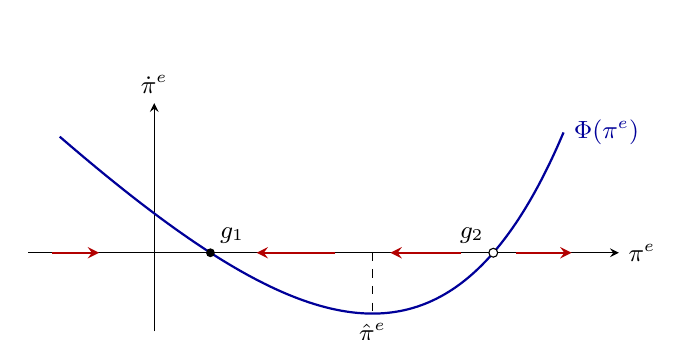
\begin{tikzpicture}[x=2cm,y=2cm,>=stealth,font=\small]
\draw[->] (-0.8,0) -- (2.95,0) node[right] {$\pi^e$};
\draw[->] (0,-0.5) -- (0,0.95) node[above] {$\dot\pi^e$};
\draw[thick,blue!60!black,domain=-0.6:2.6,samples=80,smooth] plot (\x,{0.25*exp(\x)-\x})
  node[right] {$\Phi(\pi^e)$};
\draw[dashed] (1.386,0) -- (1.386,-0.386) node[below] {$\hat\pi^e$};
\fill (0.357,0) circle (1.6pt) node[above right] {$g_1$};
\draw[fill=white] (2.153,0) circle (1.6pt) node[above left] {$g_2$};
\draw[->,thick,red!70!black] (-0.65,0) -- (-0.35,0);
\draw[->,thick,red!70!black] (1.15,0) -- (0.65,0);
\draw[->,thick,red!70!black] (1.95,0) -- (1.5,0);
\draw[->,thick,red!70!black] (2.3,0) -- (2.65,0);
\end{tikzpicture}
\end{center}

\passo{Dynamics of $m$}{$m=Ce^{-b\pi^e}$ moves opposite to $\pi^e$. From $\pi^e(0)<g_2$, $m$
converges monotonically to $m_1=G/g_1$, where $g_M=\pi=\pi^e=g_1$. From $\pi^e(0)>g_2$, $S(\pi^e)$
keeps falling as $\pi^e$ rises, so $\dot m\le-\tfrac{b\beta}{1-b\beta}[G-S(\pi^e(0))]<0$ and $m$
collapses in finite time, as in (b).}

\intuicao{Between $g_1$ and $g_2$, steady-state revenue at the expected rate exceeds $G$, so the
government needs $g_M=G/m<\pi^e$; by (4) actual inflation falls short of expectations, which are
revised down toward $g_1$. Above $g_2$ the base erodes faster than the rate rises: the required $g_M$
exceeds $\pi^e$, inflation outruns expectations, and the economy slides into hyperinflation. The
high-inflation steady state is a threshold, not an outcome, which is why the text focuses on $g_1$.}

\armadilha{If $\beta>1/b$, the factor $\beta/(1-b\beta)$ in (3) is negative and every arrow reverses:
in (b) $\pi^e$ falls forever (explosive deflation), and in (c) $g_2$ is stable and $g_1$ unstable,
the ``peculiar'' case of Romer's footnote 34.}

\refbib{Romer (2012), \S11.9, eqs.~(11.67)--(11.75), Figs.~11.8--11.10 and footnotes 33--34;
Cagan (1956).}

\checado{\texttt{check-11-22-6-16.py} re-derives (3) and (4) with sympy from the two equations,
confirms that (3) reproduces (11.75) and that $\min\Phi=\frac{\beta}{b(1-b\beta)}\ln(G/S^{\mathrm{MAX}})$;
for $C=b=1$, $\beta=\tfrac12$ it checks $G=\tfrac12$: $\Phi>0$ on a grid and the simulated $\pi^e$ passes
30 ($m<10^{-13}$) at $t\approx4.75$, before $\bar t\approx7.57$; and $G=\tfrac14$: $S(g_i)=G$, $\Phi'(g_1)<0<\Phi'(g_2)$, paths from below $g_1$
and from $(g_1,g_2)$ converge to $g_1$ and the path from above $g_2$ explodes. The solution manual
agrees with (3), with (b) and with the stability ranking in (c), but its text for (c) has a sign typo:
for $\pi^e$ outside $[g_1,g_2]$ it writes $\dot\pi^e<0$; it must be $\dot\pi^e>0$, as its own eq.~(11)
and the arrows in its figure require.}

% Romer 6.16 --- solution fragment for hardest-solutions.tex (statement not reproduced).
% Pricing solution, output effects and the mapping to Benigno's kappa re-checked by check-11-22-6-16.py.
\problema{Romer 6.16}{Flexible- and rigid-price firms}{p.~311}{Romer \S6.5--6.7; Benigno (2015) \S4}

\passo{Environment}{All variables are in logs. Aggregate demand is $y=m-p$ (eq.~(6.41) in logs). A
firm's desired price is $p^*=p+\phi y$ (eq.~(6.58) with the constant normalized to zero), that is,
$p^*=(1-\phi)p+\phi m$ (eq.~(6.61)), with $\phi>0$ so that the flexible-price equilibrium is stable
(\S6.5). Flexible-price firms set $p^f=p^*$ after observing $m$; rigid-price firms set $p^r=Ep^*$
before. $E$ is the expectation held when rigid prices are set, so a change in $m$ is
\emph{anticipated} if it is known at that moment. A fraction $q\in(0,1)$ of firms is rigid:
$p=q\,p^r+(1-q)\,p^f$. With every price flexible, $p^*=p$ forces $y=0$: natural output is $y_n=0$
and $p=m$.}

\parte{a}
\passo{Substitute the price index}{Inserting $p=q\,p^r+(1-q)\,p^f$ into $p^f=(1-\phi)p+\phi m$,
\[ p^f=(1-\phi)\big[q\,p^r+(1-q)\,p^f\big]+\phi m . \]}

\passo{Collect $p^f$}{Moving the $p^f$ terms to the left,
\[ p^f\big[1-(1-\phi)(1-q)\big]=(1-\phi)\,q\,p^r+\phi m ,\qquad
1-(1-\phi)(1-q)=q+\phi(1-q)\equiv D>0 . \]
Dividing by $D$ and using $D-\phi=(1-\phi)q$,
\[ p^f=\frac{(1-\phi)\,q\,p^r+\phi m}{q+\phi(1-q)}=p^r+\frac{\phi}{q+\phi(1-q)}\,\big(m-p^r\big). \tag{A} \]
Flexible-price firms close the fraction $\phi/D$ of the gap between money and the rigid price. Since
$D-\phi=(1-\phi)q$, $\phi/D<1$ exactly when $\phi<1$, i.e.\ when desired prices rise less than
one-for-one with the price level ($\partial p^*/\partial p=1-\phi$: strategic complementarity).}

\parte{b}
\passo{Expected flexible price}{The flexible firms' rule holds whatever $m$ turns out to be, and
expectations are linear, so $Ep^f=(1-\phi)\,Ep+\phi\,Em$. The right side is exactly the rigid
firms' rule: $Ep^f=p^r$. Each rigid firm expects to charge what the flexible firms will charge.}

\passo{Expected price level}{$p^r$ is chosen with the information behind $E$, so $Ep^r=p^r$ and
\[ Ep=q\,p^r+(1-q)\,Ep^f=q\,p^r+(1-q)\,p^r=p^r . \]}

\passo{Solve}{Substituting $Ep=p^r$ into the rigid firms' rule and dividing by $\phi>0$,
\[ p^r=(1-\phi)\,p^r+\phi\,Em\quad\Longrightarrow\quad \phi\,p^r=\phi\,Em
\quad\Longrightarrow\quad p^r=Em . \tag{B} \]
No parameter appears: rigid firms preset the price level that flexible prices would deliver given
what they know, and $Ey=Em-Ep=0$. Check against (A): with $p^r=Em$,
$Ep^f=Em+\frac{\phi}{D}(Em-Em)=Em=p^r$, as the first step requires.}

\parte{c}
\passo{Price level and output}{With (B), (A) reads $p^f=Em+\frac{\phi}{D}(m-Em)$, so
\[ \begin{aligned}
p&=q\,Em+(1-q)\Big[Em+\frac{\phi}{D}(m-Em)\Big]=Em+\frac{(1-q)\,\phi}{D}\,(m-Em),\\
y&=m-p=\Big[1-\frac{(1-q)\,\phi}{D}\Big](m-Em)=\frac{q}{q+\phi(1-q)}\,(m-Em),
\end{aligned} \tag{C} \]
because $D-(1-q)\phi=q$.}

\passo{(i) Anticipated changes}{Write $m=Em+u$, where $u\equiv m-Em$ is the part of money unknown
when rigid prices were set; by (C), $y=(q/D)\,u$ depends on $u$ alone. An anticipated change raises
$Em$ and $m$ by the same $\Delta$ and leaves $u$ unchanged: $\Delta y=0$, while $p^r$, $p^f$ and $p$
all rise by $\Delta$. Money is neutral because the rigid firms knew the change when they set their
prices, so every price incorporates it, and the flexible firms keep their relative price
$p^f-p^r=(\phi/D)\,u$ unchanged.}

\passo{(ii) Unanticipated changes}{Raising $m$ by $\Delta$ with $Em$ fixed raises $u$ by $\Delta$:
\[ \Delta y=\frac{q}{q+\phi(1-q)}\,\Delta>0,\qquad \Delta p=\frac{(1-q)\,\phi}{q+\phi(1-q)}\,\Delta<\Delta . \]
Since $D-q=\phi(1-q)>0$, $0<q/D<1$. Output absorbs part of the surprise because the fraction $q$ of
prices is stuck at $Em$; by (A), flexible firms raise their prices by $(\phi/D)\Delta$, which is less
than $\Delta$ when $\phi<1$.}

\passo{Mapping to Benigno's AS curve}{The AS curve follows from the pricing side alone. From the
price index and $Ep=p^r$, $p-Ep=(1-q)(p^f-Ep)$; and $p^f-Ep=(p^f-p)+(p-Ep)=\phi y+(p-Ep)$. Hence
\[ q\,(p-Ep)=(1-q)\,\phi\,y\quad\Longrightarrow\quad p-Ep=\frac{(1-q)\,\phi}{q}\,(y-y_n),
\qquad y_n=0 . \tag{D} \]
This is Benigno's eq.~(17), $p-p^e=\kappa\,(y-y_n)$, under the dictionary: the rigid share $q$ is
his share $\alpha$ of prices preset at $p^e$; $p^r=Ep$ is his $p^e$; $p^f$ is his $\tilde p$, whose
rule $\tilde p-p=(\sigma^{-1}+\eta)(y-y_n)$ (his eq.~(16)) is $p^*-p=\phi y$ with
$\phi=\sigma^{-1}+\eta$. Therefore $\kappa=(1-q)\phi/q=(1-\alpha)(\sigma^{-1}+\eta)/\alpha$. Romer's
\S6.5 economy is the special case $U=C-L^\gamma/\gamma$: utility is linear in $C$ ($\sigma^{-1}=0$)
and $L^\gamma/\gamma=L^{1+\eta}/(1+\eta)$ with $\eta=\gamma-1$, so $\phi=\gamma-1=\sigma^{-1}+\eta$.}

\passo{Output effect and real rigidity}{Combining (D) with the AD curve and $Ep=Em$,
$y=(m-Em)-(p-Ep)=(m-Em)-\kappa y$, so
\[ \begin{gathered}
y=\frac{m-Em}{1+\kappa},\qquad \frac{1}{1+\kappa}=\frac{q}{q+(1-q)\,\phi},\\
\frac{\partial}{\partial\phi}\Big(\frac{q}{q+\phi(1-q)}\Big)=-\frac{q\,(1-q)}{\big[q+\phi(1-q)\big]^2}<0 ,
\end{gathered} \]
which reproduces (C). Lower $\phi$ (more real rigidity) means a flatter AS (lower $\kappa$) and a
larger output response to the same surprise. Limits: as $\phi\to0$, $y\to m-Em$, so the whole
surprise goes to output although a fraction $1-q$ of firms is free to reprice (with $p^*=p$ they
choose not to); at $\phi=1$, $p^f=m$ and $y=q\,(m-Em)$; as $\phi\to\infty$, $y\to0$. With Benigno's
calibration ($\alpha=0.66$, $\sigma=0.5$, $\eta=0.2$; his \S8), $\kappa=0.34\times2.2/0.66\approx1.13$
and a 1\% money surprise raises $y$ by $1/(1+\kappa)\approx0.47\%$; keeping $\alpha=0.66$ but setting
$\phi=0.2$ gives $\kappa\approx0.10$ and $\approx0.91\%$.}

\intuicao{Real rigidity alone is neutral: with $q=0$, $y=0$ for every $\phi$ ($\kappa\to\infty$). It
magnifies nominal rigidity: when $\phi$ is small, flexible firms care mostly about their price
relative to the sticky ones, so they track the preset prices rather than money, and a small share of
preset prices freezes much of the price level (\S6.7). Anticipated money is neutral for any $q$ and
$\phi$, because no price is stuck at a stale value.}

\armadilha{(1) ``Anticipated'' refers to the information held when rigid prices are set: a change
announced after that date is a surprise here even if it is public before $m$ is realized. (2) $p^r$
is a choice, not an outcome to forecast: $Ep^r=p^r$, which is what delivers $Ep=p^r$. (3) Romer's
$\eta$ (the elasticity of demand, Benigno's $\theta$) is not Benigno's $\eta$ (the inverse Frisch
elasticity); and Benigno's $\sigma\equiv\tilde\sigma s_c$ is the intertemporal elasticity scaled by
the consumption share.}

\refbib{Romer (2012), \S6.5, eqs.~(6.41), (6.58), (6.61), and \S6.7 (real rigidity); Benigno (2015),
\S4.1, eqs.~(16)--(17), calibration in \S8.}

\checado{\texttt{check-11-22-6-16.py} solves the pricing system with sympy by brute force (without the
shortcut $Ep^f=p^r$) and confirms (A), $p^r=Em$, (C), $\partial y/\partial Em=0$ at given $u$,
$0<q/D<1$, (D) with $\kappa=(1-q)\phi/q$, its identity with $(1-\alpha)(\sigma^{-1}+\eta)/\alpha$ under
the mapping, $y=(m-Em)/(1+\kappa)$, the sign of $\partial y/\partial\phi$ and the calibration numbers.
The solution manual agrees: same $p^f$, $p^r=Em$, $y=q\,(m-Em)/[\phi+(1-\phi)q]$ and the same
real-rigidity derivative (its eq.~(19)); it does not discuss Benigno's AS.}

% Romer (2012), Problem 6.10 (pp. 308--309): solution only, the statement is not reproduced (CLAUDE.md).
% Every formula and number below is re-checked by check-6-10-6-7.py in this folder.
\problema{Romer 6.10}{Menu costs and multiple equilibria}{pp.~308--309}{Romer \S6.6--6.7}

\noindent Variables are logs. All firms face the same $p^*$, so a firm that pays the fixed cost $Z$
sets $p_i=p^*$ and one that does not keeps $p_i=0$. Firms are atomistic: one firm's choice moves
neither $f$ nor $p$, $y$ or $p^*$. Throughout, $\phi>0$ (the condition in Romer's footnote~19 for the
flexible-price equilibrium to be stable) and $m'\neq0$ (with $m'=0$ no firm has a reason to move).

\parte{a}
\passo{Eliminate $y$ from the optimal price}{Put aggregate demand $y=m'-p$ into $p^*=p+\phi y$:
\[ p^*=p+\phi(m'-p)=\phi m'+(1-\phi)\,p . \]
A firm's desired price is a weighted average of money and the price level, with weight $1-\phi$ on what the other firms charge.}
\passo{Impose $p=fp^*$ and solve for $p^*$}{Substituting $p=fp^*$,
\[ p^*=\phi m'+(1-\phi)fp^* \;\Longrightarrow\; p^*\bigl[1-(1-\phi)f\bigr]=\phi m' \;\Longrightarrow\; p^*=\frac{\phi m'}{D(f)},\qquad D(f)\equiv1-(1-\phi)f . \]
$D$ is linear in $f$ with $D(0)=1$ and $D(1)=\phi>0$, so $D>0$ on $[0,1]$ and the division is legitimate.}
\passo{Price level and output}{From $p=fp^*$ and $y=m'-p$,
\[ p=\frac{f\phi m'}{1-(1-\phi)f},\qquad y=m'-\frac{f\phi m'}{D(f)}=m'\,\frac{1-(1-\phi)f-\phi f}{D(f)}=m'\,\frac{1-f}{1-(1-\phi)f} . \]
Checks: $f=0$ gives $p=0$, $y=m'$, $p^*=\phi m'$ (output absorbs the whole shock); $f=1$ gives $p=p^*=m'$ and $y=0$ (neutrality). In between, $\partial y/\partial f=m'\,[-D(f)+(1-f)(1-\phi)]/D(f)^2=-\phi m'/D(f)^2$: each extra adjuster pushes output toward its flexible-price level.}

\parte{b}
\passo{The incentive function}{A firm that keeps $p_i=0$ loses $K(0-p^*)^2$ relative to a firm at $p^*$; a firm that adjusts loses nothing before paying $Z$. The gross gain from adjusting, as a function of the fraction $f$ of \emph{other} firms that adjust, is therefore
\[ G(f)\equiv Kp^{*2}=\frac{K\phi^2m'^2}{\bigl[1-(1-\phi)f\bigr]^2},\qquad G(0)=K\phi^2m'^2,\qquad G(1)=\frac{K\phi^2m'^2}{\phi^2}=Km'^2 . \]}
\passo{Slope and curvature}{Write $G=K\phi^2m'^2D^{-2}$ with $D'(f)=-(1-\phi)$. By the chain rule,
\[ \begin{aligned} G'(f)&=-2K\phi^2m'^2D^{-3}D'(f)=\frac{2K\phi^2m'^2(1-\phi)}{D(f)^3},\\ G''(f)&=-6K\phi^2m'^2(1-\phi)D^{-4}D'(f)=\frac{6K\phi^2m'^2(1-\phi)^2}{D(f)^4}\ \ge0 . \end{aligned} \]
As $D>0$, $\operatorname{sign}G'=\operatorname{sign}(1-\phi)$. \emph{Real rigidity, $\phi<1$:} $G$ is strictly increasing and convex, rising from $K\phi^2m'^2$ to $Km'^2$; price adjustments are strategic complements. \emph{Real flexibility, $\phi>1$:} $G$ is strictly decreasing and convex, falling from $K\phi^2m'^2$ to $Km'^2$; adjustments are strategic substitutes. At $\phi=1$, $p^*=m'$ whatever the others do and $G\equiv Km'^2$.}

\begin{center}\begin{minipage}{\linewidth}\centering
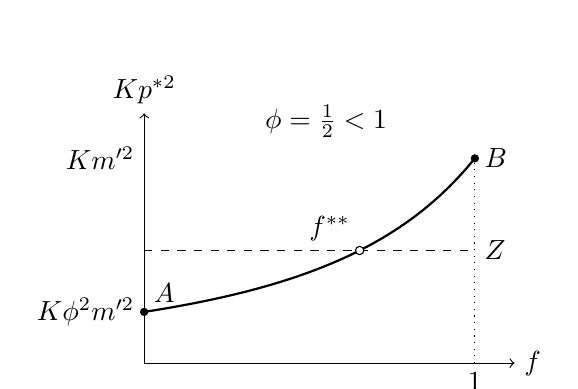
\begin{tikzpicture}[x=4.2cm,y=2.6cm]
  \draw[->] (0,0)--(1.12,0) node[right]{$f$};
  \draw[->] (0,0)--(0,1.22) node[above]{$Kp^{*2}$};
  \draw[thick,domain=0:1,samples=40] plot (\x,{0.25/((1-0.5*\x)^2)});
  \draw[dashed] (0,0.55)--(1,0.55) node[right]{$Z$};
  \draw[dotted] (1,0)--(1,1);
  \node[left] at (0,0.25){$K\phi^2m'^2$}; \node[left] at (0,1){$Km'^2$}; \node[below] at (1,0){$1$};
  \fill (0,0.25) circle (1.5pt) node[above right]{$A$};
  \fill (1,1) circle (1.5pt) node[right]{$B$};
  \draw[fill=white] (0.6516,0.55) circle (1.5pt) node[above left]{$f^{**}$};
  \node at (0.55,1.18){$\phi=\frac12<1$};
\end{tikzpicture}\qquad
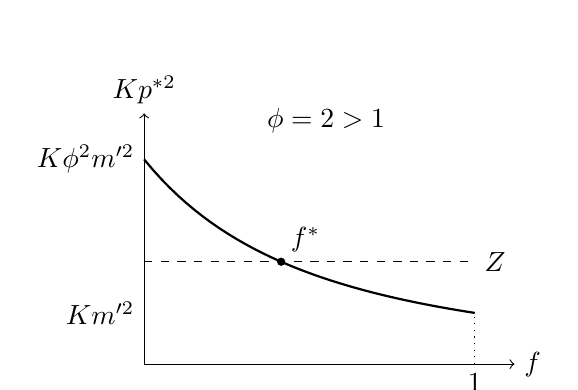
\begin{tikzpicture}[x=4.2cm,y=0.65cm]
  \draw[->] (0,0)--(1.12,0) node[right]{$f$};
  \draw[->] (0,0)--(0,4.9) node[above]{$Kp^{*2}$};
  \draw[thick,domain=0:1,samples=40] plot (\x,{4/((1+\x)^2)});
  \draw[dashed] (0,2)--(1,2) node[right]{$Z$};
  \draw[dotted] (1,0)--(1,1);
  \node[left] at (0,4){$K\phi^2m'^2$}; \node[left] at (0,1){$Km'^2$}; \node[below] at (1,0){$1$};
  \fill (0.4142,2) circle (1.5pt) node[above right]{$f^{*}$};
  \node at (0.55,4.75){$\phi=2>1$};
\end{tikzpicture}\par\smallskip
{\small $G(f)=Kp^{*2}$ with $K=m'=1$. Left, $Z=0.55$: equilibria at $A$ ($f=0$), $B$ ($f=1$) and the
unstable $f^{**}\approx0.652$. Right, $Z=2$: the unique equilibrium $f^*=\sqrt2-1\approx0.414$.}
\end{minipage}\end{center}

\parte{c}
\passo{What an equilibrium is}{Each firm takes $f$ as given; it adjusts if $G(f)>Z$, stays if $G(f)<Z$, and may do either if $G(f)=Z$. A configuration is an equilibrium when no firm wants to switch:
\[ \begin{aligned} f=1 \text{ is an equilibrium} &\iff G(1)\ge Z \iff Z\le Km'^2,\\ f=0 \text{ is an equilibrium} &\iff G(0)\le Z \iff Z\ge K\phi^2m'^2,\\ f\in(0,1) \text{ is an equilibrium} &\iff G(f)=Z , \end{aligned} \]
since in the interior case every firm is indifferent, so any split between adjusters and non-adjusters is a best response.}
\passo{Both corners at once}{Both $f=0$ and $f=1$ are equilibria iff $K\phi^2m'^2\le Z\le Km'^2$. This interval is non-empty iff $\phi^2\le1$, i.e.\ (as $\phi>0$) iff $\phi\le1$, and has positive length iff $\phi<1$. Answer: \emph{yes, exactly when $\phi<1$ and $Z\in[K\phi^2m'^2,\,Km'^2]$.} For $Z$ strictly inside, $G$ crosses $Z$ once more, at $f^{**}=\bigl(1-\phi|m'|\sqrt{K/Z}\bigr)/(1-\phi)$ (solve $G(f)=Z$ as in the last step); this third equilibrium is unstable, since just above it $G>Z$ and more firms want to adjust, and just below it $G<Z$ and adjusters want to stop. At $\phi=1$ the interval shrinks to $Z=Km'^2$, where $G\equiv Z$ and every $f\in[0,1]$ is an equilibrium.}
\passo{Neither corner}{Neither is an equilibrium iff $G(1)<Z$ and $G(0)>Z$, i.e.\ $Km'^2<Z<K\phi^2m'^2$, which is non-empty iff $\phi>1$. Answer: \emph{yes, exactly when $\phi>1$ and $Z\in(Km'^2,\,K\phi^2m'^2)$.}}
\passo{The interior equilibrium when neither corner works}{For $\phi>1$, $G$ is continuous and strictly decreasing with $G(0)>Z>G(1)$, so exactly one $f^*\in(0,1)$ has $G(f^*)=Z$. Since $D>0$,
\[ \begin{aligned} \frac{K\phi^2m'^2}{D(f^*)^2}=Z &\iff D(f^*)=\phi|m'|\sqrt{K/Z} \iff 1+(\phi-1)f^*=\phi|m'|\sqrt{K/Z}\\ &\iff f^*=\frac{\phi|m'|\sqrt{K/Z}-1}{\phi-1}, \end{aligned} \]
and $0<f^*<1\iff1<\phi|m'|\sqrt{K/Z}<\phi\iff Km'^2<Z<K\phi^2m'^2$, the same interval. At $f^*$, $|p^*|=\sqrt{Z/K}$: adjusters move by exactly the amount that makes the menu cost worth paying. With $D^*\equiv D(f^*)$ and $1-f^*=(\phi-D^*)/(\phi-1)$, output is $y^*=m'(\phi-D^*)/[(\phi-1)D^*]$, strictly between $0$ and $m'$ because $1<D^*<\phi$: money is partly neutral. The equilibrium is stable (for $f>f^*$, $G<Z$ and adjusters prefer to stay; for $f<f^*$, $G>Z$ and more firms adjust), and with $\phi>1$ the equilibrium is always unique, because $G$ is strictly monotone and the two corner conditions are incompatible.}

\begin{center}\small
\begin{tabular}{@{}lccc@{}}
\toprule
 & $Z<\min\{G(0),G(1)\}$ & $Z$ between $G(0)$ and $G(1)$ & $Z>\max\{G(0),G(1)\}$\\
\midrule
$\phi<1$ & only $f=1$ & $f=0$ and $f=1$ (and $f^{**}$ if $Z$ is interior) & only $f=0$\\
$\phi>1$ & only $f=1$ & only $f^*$ (stable) & only $f=0$\\
\bottomrule
\end{tabular}
\end{center}

\intuicao{With $\phi<1$ the desired price $p^*=\phi m'+(1-\phi)p$ leans on the others' prices. If nobody else moves, a firm's optimal change is only $\phi m'$, worth $K\phi^2m'^2$; if everybody moves it is the full $m'$, worth $Km'^2$. A menu cost between the two makes both outcomes self-fulfilling: the same nominal shock leaves the economy either rigid, with $y=m'$ (a recession when $m'<0$), or flexible, with $y=0$. Each firm's price change helps the others through aggregate demand, an externality it ignores, which is why Ball and D.~Romer (1991) read nominal rigidity as a coordination failure (Romer \S6.8). Real rigidity therefore does double duty: it shrinks the private gain from adjusting when others stay put, and it makes adjustment decisions complements. With $\phi>1$ the others' adjustment shrinks a firm's own desired change, decisions are substitutes, the equilibrium is unique, and an intermediate menu cost yields partial adjustment.}
\armadilha{(1) Letting the deviating firm's own choice move $p$ and $p^*$: with a continuum of firms its deviation has measure zero, so $p^*$ is evaluated at the others' $f$. (2) Writing the corner conditions with strict inequalities only: an indifferent firm may do either, so the intervals are closed and $f=1$ survives at $Z=Km'^2$. (3) Reading $G(0)<G(1)$ as multiplicity for every $Z$: it needs $Z\in[K\phi^2m'^2,Km'^2]$, and outside that interval the equilibrium is unique even with $\phi<1$. (4) Treating only expansions: everything depends on $m'^2$ and $|m'|$, so a contraction is the mirror image.}
\refbib{Romer (2012), \S6.6--6.7 (pp.~275--286): the incentive to adjust, real rigidity and eq.~(6.58); \S6.8 (from p.~286): coordination failure. Ball and D.~Romer (1991), ``Sticky Prices as Coordination Failure,'' \emph{American Economic Review} 81, 539--552.}
\checado{\texttt{check-6-10-6-7.py} re-derives $p^*$, $p$, $y$, $G$, $G'$, $G''$ and $f^*$ with sympy, and with $K=m'=1$ confirms the interval $[0.25,1]$ and three equilibria at $Z=0.55$ for $\phi=\frac12$ ($f^{**}=0.6516$), and the unique $f^*=y^*=\sqrt2-1$ at $Z=2$ for $\phi=2$, by scanning $G(f)-Z$ on a grid; the same scan confirms both interval claims, and uniqueness whenever $\phi>1$, on a grid of $Z$ for $\phi\in\{0.5,0.75,1.5,2\}$. The solution manual agrees on every part; it states the intervals with strict inequalities and does not solve for the interior equilibrium.}

% Romer (2012), Problem 6.7 (p. 308): solution only, the statement is not reproduced (CLAUDE.md).
% Every formula and number below is re-checked by check-6-10-6-7.py in this folder.
\problema{Romer 6.7}{The liquidity trap}{p.~308}{Romer \S6.4; Benigno (2015) \S9}

\noindent With $\bar y\equiv0$, $y$ is the output gap, $i$ the nominal rate and $i-\pi$ the real rate in the
traditional IS curve. The rule (6.26) is a continuously differentiable $r(y,\pi)$ with $r_1>0$ and
$r_2>0$. Two regularity conditions, both true for the linear rule used below, are assumed: for every
$\pi$ the equation $\theta y+r(y,\pi)=0$ has a solution, and the kink $(\tilde y,\tilde\pi)$ exists (the
statement presupposes it). The figures use $r=c+ay+b\pi$ with $\theta=2$, $a=1$, $b=3$, $\lambda=\frac12$,
and $c=-9$ (then $\tilde y>0$) or $c=4.5$ (then $\tilde y<0$); every result is proved for a general $r$.

\parte{a}
\passo{Combine the IS curve and the constrained rule}{The IS curve says $\theta y=\pi-i$. Substituting $i=\max[0,\pi+r(y,\pi)]$ and using $-\max\{u,v\}=\min\{-u,-v\}$,
\[ \theta y=\pi-\max\bigl[0,\ \pi+r(y,\pi)\bigr]=\min\bigl[\pi,\ -r(y,\pi)\bigr]. \]
This single equation is the AD curve. Equivalently, the real rate is $i-\pi=\max[r(y,\pi),-\pi]$: what the bank wants, unless that lies below the floor $-\pi$ imposed by $i\ge0$.}
\passo{The two branches}{A minimum equals $\theta y$ iff one term equals $\theta y$ and the other is not smaller, so a point is on the AD curve iff
\[ \begin{aligned} &\text{(L), zero bound binding:} && \theta y=\pi && \text{and} && \pi+r(y,\pi)\le0,\\ &\text{(U), zero bound slack:} && \theta y+r(y,\pi)=0 && \text{and} && \pi+r(y,\pi)\ge0 . \end{aligned} \]
At the kink both hold: $\theta\tilde y=\tilde\pi$ and $\theta\tilde y+r(\tilde y,\tilde\pi)=0$.}
\passo{Which branch applies where}{On the line $\pi=\theta y$ let $h(y)\equiv\theta y+r(y,\theta y)$; then $h'(y)=\theta+r_1+\theta r_2>0$ and $h(\tilde y)=0$, so a point of the line is on (L) iff $h(y)\le0$, i.e.\ iff $y\le\tilde y$, i.e.\ iff $\pi\le\tilde\pi$. On (U), $y=Y(\pi)$, the unique root of $\theta y+r(y,\pi)=0$ (its left side rises in $y$ at rate $\theta+r_1>0$), with $Y(\tilde\pi)=\tilde y$ and, by implicit differentiation, $Y'(\pi)=-r_2/(\theta+r_1)<0$. Since $r(Y,\pi)=-\theta Y$, the side condition of (U) is $k(\pi)\equiv\pi-\theta Y(\pi)\ge0$; as $k'(\pi)=1+\theta r_2/(\theta+r_1)>0$ and $k(\tilde\pi)=0$, it holds iff $\pi\ge\tilde\pi$. Hence each $\pi$ has exactly one output level on the AD curve:
\[ y=A(\pi)\equiv\begin{cases} \pi/\theta, & \pi\le\tilde\pi\quad\text{(nominal rate at zero)},\\ Y(\pi), & \pi\ge\tilde\pi\quad\text{(rule (6.26) operative)}. \end{cases} \]}
\passo{Slopes and the kink}{In the $(y,\pi)$ plane, differentiating $\theta y+r(y,\pi)=0$ and $\theta y=\pi$,
\[ \left.\frac{d\pi}{dy}\right|_{\text{U}}=-\frac{\theta+r_1}{r_2}<0,\qquad \left.\frac{d\pi}{dy}\right|_{\text{L}}=\theta>0 . \]
Above $\tilde\pi$ the AD curve slopes down as in Romer's Figure~6.9: lower inflation makes the bank cut the real rate. Below $\tilde\pi$ it bends back: with $i=0$ the real rate is $-\pi$, so lower inflation \emph{raises} it and output falls. $A$ rises on $(-\infty,\tilde\pi]$ and falls on $[\tilde\pi,\infty)$, so $\tilde y=\max_\pi A(\pi)$ is the most output any inflation rate can support. As $h$ is increasing with $h(\tilde y)=0$, $\tilde y>0\iff h(0)<0\iff r(0,0)<0$. If $\pi^H$ is the inflation rate at which the rule is neutral, $r(0,\pi^H)=0$, then $r_2>0$ makes this equivalent to $\pi^H>0$, a positive nominal rate $i=\pi^H$ at the targeted steady state. With a natural rate in the IS curve, $\theta y=r^n+\pi-i$, and a rule neutral at $r(0,\pi^H)=r^n$, the kink solves $\theta y-r^n+r(y,\theta y-r^n)=0$, so $\tilde y>0\iff r(0,-r^n)<r(0,\pi^H)\iff r^n+\pi^H>0$: $\tilde y<0$ is the slump of Krugman (1998) and Benigno (2015, \S9), in which $r^n$ has fallen so far that the targeted steady state would need $i<0$.}

\begin{center}\begin{minipage}{\linewidth}\centering
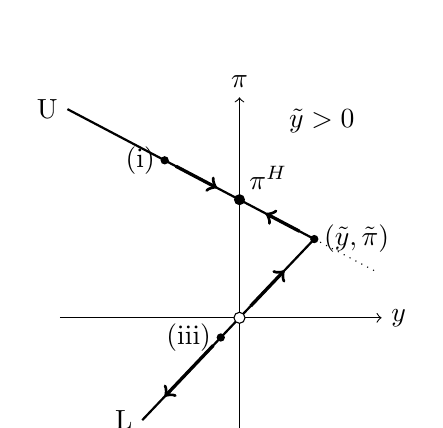
\begin{tikzpicture}[x=0.95cm,y=0.5cm]
  \draw[->] (-2.4,0)--(1.9,0) node[right]{$y$};
  \draw[->] (0,-2.8)--(0,5.6) node[above]{$\pi$};
  \draw[thick] (-1.3,-2.6)--(1,2)--(-2.3,5.3);
  \draw[dotted] (1,2)--(1.8,1.2);
  \draw[->,very thick] (-0.85,3.85)--(-0.3,3.3);
  \draw[->,very thick] (0.8,2.2)--(0.35,2.65);
  \draw[->,very thick] (0.15,0.3)--(0.6,1.2);
  \draw[->,very thick] (-0.35,-0.7)--(-1,-2);
  \fill (0,3) circle (2pt) node[above right]{$\pi^H$};
  \draw[fill=white] (0,0) circle (2pt);
  \fill (1,2) circle (1.5pt) node[right]{$(\tilde y,\tilde\pi)$};
  \fill (-1,4) circle (1.5pt) node[left]{(i)};
  \fill (-0.25,-0.5) circle (1.5pt) node[left]{(iii)};
  \node[left] at (-2.3,5.3){U}; \node[left] at (-1.3,-2.6){L};
  \node at (1.1,5){$\tilde y>0$};
\end{tikzpicture}\qquad
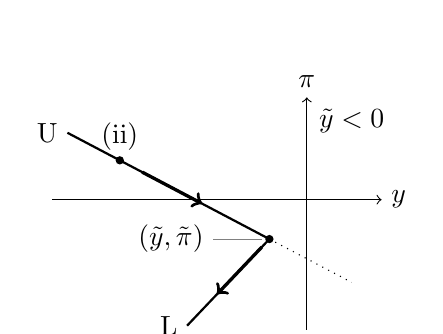
\begin{tikzpicture}[x=0.95cm,y=0.5cm]
  \draw[->] (-3.4,0)--(1,0) node[right]{$y$};
  \draw[->] (0,-3.3)--(0,2.6) node[above]{$\pi$};
  \draw[thick] (-1.6,-3.2)--(-0.5,-1)--(-3.2,1.7);
  \draw[dotted] (-0.5,-1)--(0.6,-2.1);
  \draw[->,very thick] (-2.2,0.7)--(-1.4,-0.1);
  \draw[->,very thick] (-0.6,-1.2)--(-1.2,-2.4);
  \fill (-0.5,-1) circle (1.5pt);
  \draw[gray] (-0.6,-1)--(-1.25,-1) node[left,black]{$(\tilde y,\tilde\pi)$};
  \fill (-2.5,1) circle (1.5pt) node[above]{(ii)};
  \node[left] at (-3.2,1.7){U}; \node[left] at (-1.6,-3.2){L};
  \node at (0.6,2){$\tilde y<0$};
\end{tikzpicture}\par\smallskip
{\small AD curves for the linear rule (dotted: where the rule alone would put AD without the zero bound).
Motion along AD follows $\dot\pi=\lambda y$: down where $y<0$, up where $y>0$. Filled dot: the stable
steady state $\pi^H$; open dot: the unstable trap $\pi=y=i=0$. Starting points of cases (i)--(iii) marked.}
\end{minipage}\end{center}

\parte{b}
\passo{A phase line on the AD curve}{Inflation is predetermined ($\dot\pi$ is finite, so $\pi$ cannot jump), while $y$ moves instantly to keep the economy on the AD curve. So $y(t)=A(\pi(t))$ and the model reduces to one autonomous equation,
\[ \dot\pi=F(\pi)\equiv\lambda A(\pi). \]
$F$ is continuous and piecewise $C^1$, hence locally Lipschitz: the solution is unique, $\pi$ moves monotonically, and it never crosses a zero of $F$. The zeros are the steady states, $A(\pi)=0$: on (L), $\pi/\theta=0$ gives $\pi=0$, admissible iff $0\le\tilde\pi$, i.e.\ $\tilde y\ge0$; on (U), $Y(\pi)=0$ means $r(0,\pi)=0$, i.e.\ $\pi=\pi^H$, admissible iff $\pi^H\ge\tilde\pi$, which requires $\tilde y=Y(\tilde\pi)\ge0$ because $Y$ is decreasing.}
\passo{A trap no interest-rate rule can escape}{Since $\theta y=\min[\pi,-r]\le\pi$, every $\pi<0$ gives $y\le\pi/\theta<0$ and $\dot\pi<0$, \emph{whatever the rule}: with $i\ge0$ the real rate is at least $-\pi>0$.}
\passo{Steady states and stability}{If $\tilde y>0$ and $Y$ turns negative at high inflation (true for the linear rule, and implied by the data of case (i)), there are two steady states, $0<\tilde\pi<\pi^H$, the last inequality because $Y(\tilde\pi)=\tilde y>0=Y(\pi^H)$ with $Y$ decreasing. $F<0$ on $(-\infty,0)$; $F>0$ on $(0,\pi^H)$, because $A=\pi/\theta>0$ on $(0,\tilde\pi]$ and $A=Y>0$ on $[\tilde\pi,\pi^H)$; and $F<0$ on $(\pi^H,\infty)$. So $\pi^H$ is stable with basin $(0,\infty)$, while the liquidity-trap steady state $\pi=y=i=0$ is unstable; locally, $F'(\pi^H)=-\lambda r_2/(\theta+r_1)<0<F'(0)=\lambda/\theta$. If $\tilde y<0$, $A(\pi)\le\tilde y<0$ for every $\pi$ and there is no steady state at all. (At $\tilde y=0$ the two merge at the kink, which attracts from above and repels from below.)}
\passo{Case (i): $\tilde y>0$, $\pi(0)>\tilde\pi$, $y(0)<0$}{The economy starts on (U) with $Y(\pi(0))<0<\tilde y=Y(\tilde\pi)$, so $\pi^H\in(\tilde\pi,\pi(0))$ by continuity and monotonicity of $Y$. On $(\pi^H,\infty)$, $F<0$: inflation falls monotonically, cannot cross $\pi^H$ and, being bounded below, converges to a zero of $F$, which can only be $\pi^H$. Output $y=Y(\pi)$ rises monotonically to $0$, and the nominal rate stays positive throughout because $\pi>\tilde\pi$: an ordinary disinflation, in which the bank cuts the real rate as inflation falls. Near $\pi^H$ the gap decays at rate $\lambda r_2/(\theta+r_1)$; with the linear rule, $Y(\pi)=-b(\pi-\pi^H)/(\theta+a)$, so exactly $\pi(t)=\pi^H+(\pi(0)-\pi^H)e^{-\mu t}$ and $y(t)=y(0)e^{-\mu t}$, with $\mu=\lambda b/(\theta+a)$.}
\passo{Case (ii): $\tilde y<0$, $\pi(0)>\tilde\pi$}{Here $y(0)=Y(\pi(0))\le\tilde y<0$. \emph{Phase 1, on (U).} $\dot\pi=\lambda Y(\pi)\le\lambda\tilde y<0$, so inflation falls at least at speed $\lambda|\tilde y|$ and reaches $\tilde\pi$ at some $t_1\le(\pi(0)-\tilde\pi)/(\lambda|\tilde y|)$, while output $Y(\pi)$ \emph{rises} toward $\tilde y$ because the bank keeps cutting $i$. \emph{Phase 2, on (L), $t\ge t_1$.} Now $i=0$, $y=\pi/\theta$ and $\dot\pi=(\lambda/\theta)\pi$ with $\pi(t_1)=\tilde\pi=\theta\tilde y<0$, so
\[ \pi(t)=\tilde\pi\,e^{(\lambda/\theta)(t-t_1)}\to-\infty,\qquad y(t)=\tilde y\,e^{(\lambda/\theta)(t-t_1)}\to-\infty . \]
Inflation falls for ever; output first recovers, then collapses. With the linear rule, phase 1 is case (i)'s formula aimed at the unreachable $\pi^H=-c/b<\tilde\pi$, so $t_1=\mu^{-1}\ln[(\pi(0)-\pi^H)/(\tilde\pi-\pi^H)]$.}
\passo{Case (iii): $\tilde y>0$, $\pi(0)<\tilde\pi$, $y(0)<0$}{The economy starts on (L), so $y(0)=\pi(0)/\theta<0$ forces $\pi(0)<0$: it starts below the unstable steady state. For all $t$, $\dot\pi=(\lambda/\theta)\pi$, hence $\pi(t)=\pi(0)e^{(\lambda/\theta)t}$ and $y(t)=\pi(t)/\theta$, both falling without bound with $i=0$ throughout; $\pi^H$ exists but is never reached. Had $0<\pi(0)<\tilde\pi$ (so $y(0)>0$), inflation would have risen, crossed $\tilde\pi$ in finite time and converged to $\pi^H$ along (U): $\pi=0$ is the watershed between recovery and collapse.}

\begin{center}\begin{minipage}{\linewidth}\centering
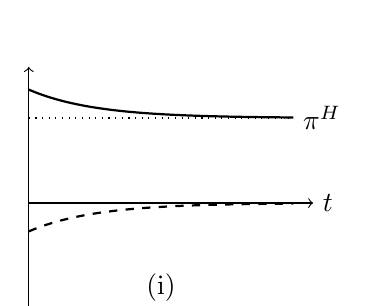
\begin{tikzpicture}[x=0.42cm,y=0.36cm]
  \draw[->] (0,0)--(8.6,0) node[right]{$t$}; \draw[->] (0,-4)--(0,4.8);
  \draw[dotted] (0,3)--(8,3) node[right]{$\pi^H$};
  \draw[thick,domain=0:8,samples=50] plot (\x,{3+exp(-0.5*\x)});
  \draw[thick,dashed,domain=0:8,samples=50] plot (\x,{-exp(-0.5*\x)});
  \node at (4,-3){(i)};
\end{tikzpicture}\quad
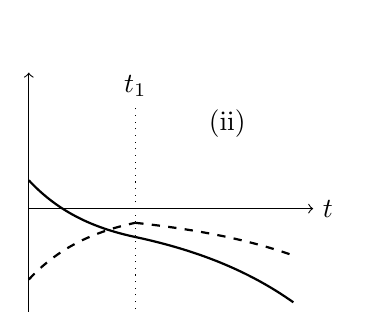
\begin{tikzpicture}[x=0.42cm,y=0.36cm]
  \draw[->] (0,0)--(8.6,0) node[right]{$t$}; \draw[->] (0,-4)--(0,4.8);
  \draw[dotted] (3.2189,-4)--(3.2189,3.6) node[above]{$t_1$};
  \draw[thick,domain=0:3.2189,samples=40] plot (\x,{-1.5+2.5*exp(-0.5*\x)});
  \draw[thick,domain=3.2189:8,samples=40] plot (\x,{-exp(0.25*(\x-3.2189))});
  \draw[thick,dashed,domain=0:3.2189,samples=40] plot (\x,{-2.5*exp(-0.5*\x)});
  \draw[thick,dashed,domain=3.2189:8,samples=40] plot (\x,{-0.5*exp(0.25*(\x-3.2189))});
  \node at (6,3){(ii)};
\end{tikzpicture}\quad
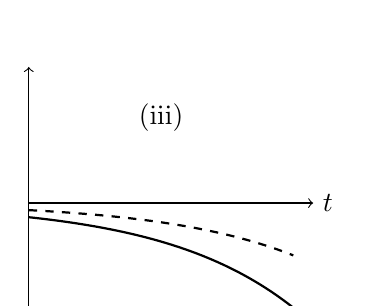
\begin{tikzpicture}[x=0.42cm,y=0.36cm]
  \draw[->] (0,0)--(8.6,0) node[right]{$t$}; \draw[->] (0,-4)--(0,4.8);
  \draw[thick,domain=0:8,samples=50] plot (\x,{-0.5*exp(0.25*\x)});
  \draw[thick,dashed,domain=0:8,samples=50] plot (\x,{-0.25*exp(0.25*\x)});
  \node at (4,3){(iii)};
\end{tikzpicture}\par\smallskip
{\small Time paths for the linear rule: $\pi(t)$ solid, $y(t)$ dashed. (i) $c=-9$, $\pi(0)=4$, so
$\pi^H=3$ and $\mu=\frac12$; (ii) $c=4.5$, $\pi(0)=1$, $t_1=2\ln5\approx3.22$; (iii) $c=-9$, $\pi(0)=-\frac12$.}
\end{minipage}\end{center}

\passo{The way out: raise expected inflation}{Suppose the bank can make expected inflation exceed current inflation by $\Delta>0$ through a credible promise of higher future prices. The real rate in the IS curve becomes $i-\pi-\Delta$, the rule still targets it, $i=\max[0,\pi+\Delta+r(y,\pi)]$, and the first step of (a) now gives
\[ \theta y=\min\bigl[\pi+\Delta,\ -r(y,\pi)\bigr]. \]
Branch (U) is unchanged, but (L) shifts out to $y=(\pi+\Delta)/\theta$: the repelling point moves from $\pi=0$ to $\pi=-\Delta$, and any $\pi>-\Delta$ on (L) now has $y>0$ and $\dot\pi>0$. In case (iii), a promise $\Delta>-\pi(t)$ turns the spiral into a recovery at $i=0$ without touching $r(\cdot)$, and it need only last until $\pi>0$, when the economy has entered the basin $(0,\infty)$ of $\pi^H$. In case (ii) no temporary promise is enough, since $A<0$ at every $\pi$: the rule's own steady state, if any, needs $i<0$. What works there is a permanently higher target, $\pi^H>0$ (with a natural rate, $\pi^H>-r^n$), which moves the kink to $\tilde y>0$ and creates the basin of recovery, plus a temporary $\Delta$ if inflation is already negative.}

\intuicao{Above $\tilde\pi$ the rule is stabilising: lower inflation brings a lower real rate, higher output and, through $\dot\pi=\lambda y$, an end to disinflation. Below $\tilde\pi$ the nominal rate is stuck at zero and the real rate is $-\pi$, so the feedback changes sign: lower inflation raises the real rate, depresses output and lowers inflation further. This deflationary spiral is why $\pi=0$ is a steady state that repels, and why the rule $r(\cdot)$, however aggressive, is powerless on (L). The lever left is the wedge between expected and current inflation, which is Benigno's (2015, \S9) point: in his AD equation (21) the real rate is $i-(\bar p-p)$, so raising the long-run price level $\bar p$ lowers it even at $i=0$ and shifts both AD and its zero-bound version AD$_0$ outward. In Romer's model expected inflation is tied to current inflation, and $\Delta$ is exactly the missing $\bar p$ channel.}
\armadilha{(1) Drawing the zero-bound branch as a continuation of the downward-sloping AD: below $\tilde\pi$ the AD bends back. (2) Expecting a more aggressive rule to rescue case (iii): on (L) the rule is inoperative, and for $\pi<0$ every rule gives $y\le\pi/\theta<0$. (3) Treating $y(0)$ as a free initial condition: $y$ is pinned by $\pi(0)$ through $A$, so the conditions on $y(0)$ in (i) and (iii) only place $\pi(0)$ relative to $\pi^H$ and $0$. (4) Claiming that output falls monotonically in (ii): it first rises along (U).}
\refbib{Romer (2012), \S6.4 (pp.~255--267): eqs.~(6.22)--(6.23), the rule (6.26) and Figures 6.8--6.9; \S11.6 on the zero lower bound. Benigno (2015), \S9 (``Liquidity trap'') and the AD equation (21), p.~509. Krugman (1998), cited there.}
\checado{\texttt{check-6-10-6-7.py} confirms the identity $\pi-\max[0,\pi+r]=\min[\pi,-r]$, solves the AD equation by bisection and matches the piecewise $A(\pi)$ (kink $(1,2)$ and $\pi^H=3$ for $c=-9$; kink $(-0.5,-1)$ for $c=4.5$), confirms the branch split at $\tilde\pi$ and the slope $-(\theta+r_1)/r_2$ on a nonlinear rule, checks the kink formulas with $r^n$ and with $\Delta$ in sympy, and integrates $\dot\pi=\lambda A(\pi)$ by RK4: (i) converges to $\pi^H$ along the closed form, (ii) crosses $\tilde\pi$ at $t_1=2\ln5$ with peak output $\tilde y$ and then diverges, (iii) diverges, $\pi(0)=0.1$ recovers, no linear rule tried escapes from $\pi<0$, and a temporary $\Delta=1$ rescues case (iii) while $\Delta=0.3$ does not. The solution manual agrees on (a) and all three cases (it works in $(y,r)$ space); it does not discuss the steady state at $\pi=0$ or the way out.}


\end{document}
